\section{Progress Since the Previous Long-Range Plan; Current Status}
\label{Sec:Progress}
Enormous progress has been made in the experimental and theoretical study of hot QCD matter since the 
2007 Long Range Plan\cite{LRP:2007}. A new energy frontier at the LHC, in concert with a wide variety
of experimental tools honed at RHIC, enabled rapid yet refined
analyses of the highest energy heavy ion collisions studied to date.
At the same time, upgrades to both RHIC and its experiments allowed
not only exploration of a new low-energy regime but also greatly improved
experimental sensitivity at RHIC's top energy. In combination with increasingly sophisticated
theoretical models, these developments have led to new insights into the behavior
of nuclear matter under extreme conditions. This section details
the advances in both the experimental facilities
and the results derived from them since the last Long Range Plan.


\subsection{Facilities Status}
\label{Sec:Facilities}
Collisions of heavy nuclei at ultra-relativistic energies are studied at two facilities: the Relativistic Heavy Ion Collider (RHIC) at Brookhaven National Laboratory, and (since 2010) the Large Hadron Collider (LHC) in Geneva, Switzerland. The impressive experimental progress in the field since the 2007 Long Range Plan that is presented in what follows has been made possible by the outstanding performance of these two facilities. 

RHIC began operations in 2000 with the capability of colliding nuclei from deuterons to Au at center-of-mass energies of 
200 GeV per nucleon pair.\footnote{RHIC also can collide  polarized protons at energies up to $\sqrt{s}=510$~GeV. This unique capability forms the basis of the RHIC Spin program\cite{Aschenauer:2015eha} discussed in the Cold QCD Town Meeting White Paper.}
Recommendation IV of the 2007 Long Range Plan endorsed the ``RHIC II'' luminosity upgrade, envisioned as a 10-20 fold increase above the design luminosity of $2 \times 10^{26}\ \mathrm{cm^{-2} s^{-1}}$ for full energy \AuAu\ collisions. 
While this upgrade was a high priority of the nuclear science community, the then-estimated cost of $\sim$\$150M drove a proposed funding profile that would have provided this capability no earlier than 2016. Remarkably, breakthroughs in both transverse and longitudinal stochastic cooling by the BNL Collider-Accelerator Department scientists have made it possible to achieve luminosities well above the RHIC II specification 3 years earlier at roughly 15\% of the cost projected in 2007. The new RHIC luminosity performance is shown in the left panel of Figure~\ref{Fig:RHICLum},
demonstrating that the \AuAu\ luminosity from the 2014 RHIC run routinely exceeded RHIC II luminosities. As a result, the integrated luminosity for \AuAu\ collisions acquired in Run 14 significantly exceeds the sum of {\em all} previous RHIC runs\cite{RHICPerformance}, as shown in the right panel of Figure~\ref{Fig:RHICLum}.
\begin{figure}[ht]
\centerline{
\includegraphics[width=0.60\textwidth]{fig/RHICLuminosity.png}
\includegraphics[width=0.40\textwidth]{fig/RhicIntegratedLuminosityAA.png}
}
\caption[RHIC luminosity, past and present]{Left: the luminosity for $\sqrt{s_{NN}}=200$~GeV \AuAu\ collisions as a function of time in the 2014 RHIC Run, compared to RHIC and RHIC II design luminosity.
Right: the integrated luminosity for all RHIC heavy ions runs.
}
\label{Fig:RHICLum}
\end{figure}

RHIC's capabilities were extended in 2011 with the commissioning 
of an Electron Beam Ion Source\cite{Alessi:2010zz} 
(EBIS)\footnote{EBIS was partially funded by NASA for the study of space radiation effects on extended human space missions
at NASA's Space Radiation Laboratory located at BNL.}, 
which replaced the aging Tandem Accelerator as a source for injection into the AGS/RHIC accelerator chain. The new physics enabled by EBIS was demonstrated in definitive fashion in 2012, when RHIC became the first collider to produce \UU\ collisions. 
The intrinsic deformation of the ${}^{238}$U nucleus provides a valuable tool 
in constraining models of the initial state energy deposition 
and separating the effects from overlap geometry and quantum fluctuations in the initial state on the hydrodynamic flow in the final state.
Similarly, in 2014 RHIC provided the first \HeAu\ collisions to study the development of odd-harmonic hydrodynamic flow resulting from the three nucleons in ${}^3$He. Both of these developments are described in more detail in Section~\ref{Sec:Flow}.

Another demonstration of the flexibility of the RHIC is the Beam Energy Scan (BES) in search of the QCD critical point.  Phase I of this campaign was conducted in 2010, 2011 and 2014. In addition to full energy \AuAu\ collisions at $\sqrt{s_{NN}} = 200$~GeV, data were taken for \AuAu\ collisions at 
$\sqrt{s_{NN}}$ 62.4 GeV, 39 GeV, 27 GeV, 19.6 GeV, 14.5 GeV, 11.5 GeV and 7.7 GeV. As discussed in more detail in Section~\ref{Sec:BES} this range of energies explores the region in the QCD phase diagram (as a function of baryon chemical potential $\mu_B$ and temperature) in which it is predicted that the smooth cross-over transition observed at the highest RHIC energies transforms into a first-order phase transition. The capability to explore this regime is a unique feature of RHIC.

Both the PHENIX\cite{PHENIX} and the STAR\cite{STAR} experiments at RHIC have undergone significant upgrades since the last Long Range Plan. PHENIX extended its measurement capabilities at forward angles with a Muon Piston Calorimeter\cite{Chiu:2007zy}, which is now being upgraded with a pre-shower detector\cite{Campbell:2013zw}. 
STAR increased its data acquisition and triggering capabilities via the DAQ1000\cite{STAR:DAQ1000} and High Level Trigger\cite{STAR:HLT}
projects. The Time of Flight\cite{STAR:TOF} detector greatly extended their particle identification capabilities
and together with the muon telescope  detector\cite{Ruan:2009ug} significantly improved its capabilities to study physics in the di-lepton channel.
Both experiments installed silicon-based tracking systems for vertexing and heavy-flavor detection, 
the VTX\cite{Nouicer:2008pf,Taketani:2010zz} and FVTX\cite{Aidala:2013vna} for PHENIX and the HFT\cite{Kapitan:2008kk,Qiu:2014dha} for STAR. These new capabilities, together with the greatly increased RHIC luminosity, are the realization of the RHIC II upgrade envisioned in the 2007 Long Range Plan.

\begin{figure}[!htb]
\begin{center}
\includegraphics[width=0.8\textwidth]{fig/LHC_chain.png}
\caption{Schematic view of the LHC accelerator complex}
\label{fig:lhc_complex}
\end{center}
\end{figure}
 
Late 2009 marked the beginning of CERN LHC operations, with a pilot run providing
first proton+proton collisions with collision energies of 0.9 and 2.36~TeV. 
The first year of LHC physics running began with p+p running at 7~TeV in April 2010 and 
ended with first Pb+Pb collisions at $\rootsNN = 2.76$~TeV in November and 
December, increasing the center-of-mass energy explored in heavy ion collisions by a factor 
of 14 compared to RHIC. The heavy ion program, which was foreseen in LHC
planning from the beginning, uses most of the elements of the LHC 
accelerator chain shown in in Figure~\ref{fig:lhc_complex}, beginning
from the electron cyclotron resonance ion source and linear accelerator, 
which provide $^{208}$Pb ions stripped to Pb$^{29+}$ at 4.2 MeV/n.
After further carbon foil stripping, bunch shaping and 
electron cooling in the CERN Low Energy Ion Ring (LEIR),  
Pb$^{54+}$ ion bunches are sent to the CERN PS, accelerated and fully stripped,
yielding Pb$^{82+}$.  After acceleration in the SPS to to 177 GeV/n,
injection and acceleration in the LHC are the final steps. 
Using 120 colliding bunches for each beam, a peak luminosity of 
$3 \times 10^{25} \mathrm{cm}^{-2} \mathrm{s}^{-1}$ was achieved 
in the 2010 LHC run.  This corresponds to an 
integrated luminosity of 7~$\mu \mathrm{b}^{-1}$ delivered to each
of three interaction regions for the ALICE, ATLAS and CMS experiments
participating in heavy-ion data taking. 

\begin{figure}[ht]
\centerline{
\includegraphics[width=0.55\textwidth]{fig/IntegratedLumPbPb.png}
\includegraphics[width=0.45\textwidth]{fig/IntegratedLumpPbII.png}
}
\caption[LHC luminosity]{Left: Delivered and recorded integrated luminosities at 
CMS for $\sqrt{s_{NN}}=2.76$~GeV \PbPb\ collisions as a function of 
time for the 2010 and 2011 LHC Pb+Pb runs.
Right: Integrated luminosity for the $\sqrt{s_{NN}}=5.02$~TeV p+Pb 2013 LHC Run.
}
\label{Fig:LHCLum}
\end{figure}
For the November--December 2011 run, an increase in the number of 
colliding bunches to 360 per ring, as well as improved focusing, allowed 
an increase in peak luminosity by a factor of 15--20, reaching close to 
design collision rates. The total delivered luminosity per interaction region 
was about 150~$\mu \mathrm{b}^{-1}$, with delivered and 
recorded luminosity in CMS shown in Figure~\ref{Fig:LHCLum} (left).

The third heavy-ion data taking period in early 2013 provided proton+lead and lead+proton
collisions at 5.02~TeV, following a pilot run in fall 2012.
Although this mode of operation was not foreseen in the baseline design of the LHC,
beams were commissioned in 10 days. The physics requirements of all experiments 
were met in three weeks of physics running, resulting in an integrated luminosity of up to 
35~$n \mathrm{b}^{-1}$ and record intensity levels, Figure~\ref{Fig:LHCLum} (right).  
A p+p reference data set at 2.76~TeV was also recorded. 

All four major LHC detectors have participated in heavy-ion data taking
in the 2009--2013 period (Run I), with ALICE, ATLAS and CMS taking p+p, p+Pb and
Pb+Pb data, and LHCb taking p+p and p+Pb data. ALICE\cite{ALICE} has been optimized
for heavy-ion operations, with large kinematic coverage, in particular at low 
transverse momenta, and charged particle identification over a wide 
momentum range using a variety of techniques. ATLAS\cite{ATLAS} and CMS\cite{CMS} are general purpose
collider detectors, with a particular focus on high data taking rates, full 
azimuthal coverage over a wide rapidity range and high resolution at very 
high transverse momenta. Although designed for discovery physics in p+p 
collisions, the high granularity of ATLAS and CMS makes them suitable
for heavy-ion collisions as well, in particular for high momentum 
probes where they complement the strengths of the ALICE detector. The heavy-ion 
related program of LHCb\cite{LHCb} was focussed on quarkonia measurements in p+Pb 
collisions at forward rapidities.

\subsection{Hydrodynamics and Collective Flow}
\label{Sec:Flow}

The initial discovery of strong elliptic flow at RHIC~\cite{Ackermann:2000tr} 
and the characteristic hydrodynamic signature of mass ordering 
in the medium response~\cite{Adler:2003kt,Kolb:2003dz} focussed a great deal 
of attention on improving the relativistic hydrodynamic description 
of the quark-gluon plasma. (See Ref.~\cite{Gale:2013da} for a recent review.)
One of the most important recent discoveries made in heavy ion collisions since the last Long-Range Plan
is the persistence of density fluctuations from the initial state. 
Recent work~\cite{Mishra:2007tw,Voloshin:2003ud,Takahashi:2009na,Sorensen:2010zq,Alver:2010gr,Qiu:2011iv,ALICE:2011ab,Adare:2011tg,ATLAS:2012at,Adamczyk:2013waa}
demonstrates that these fluctuations survive through the expansion of the fireball and appear as correlations between produced particles.
Most previous approaches had approximated the incoming nuclei as smooth spheres and the initial overlap region as an ellipse. The survival of density and geometry fluctuations was first hinted at in measurements of cumulants related to the shape of the elliptic flow distribution~\cite{Adler:2002pu,Miller:2003kd}. The picture started to become more clear after measurements were made in Cu+Cu collisions where the relative fluctuations were more prominent in the smaller system~\cite{Alver:2008zza}.  Ultimately, a new paradigm emerged as the structure of the initial state was found to play a central role 
in determining the azimuthal anisotropies with respect to the event plane angles $\Phi_n$, parameterized in terms of transverse momentum $p_T$ and azimuthal angle $\phi$ as
\begin{equation}
\label{Eq:vnDef}
\frac{d^2n}{p_T dp_T d\phi}
\sim
1 
+ 2 v_2(p_T) \cos 2 (\phi - \Phi_2)
+ 2 v_3(p_T) \cos 3 (\phi - \Phi_3)
+ 2 v_4(p_T) \cos 4 (\phi - \Phi_4)
+ \dots
\end{equation}
Previous measurements that were focused almost exclusively on the dominant $v_2$ were generalized to $v_n$, a spectrum carrying information about both the initial densities in the collision and the dissipative properties of the subsequent plasma phase~\cite{Heinz:2013th}. The survival of the initial state fluctuations is related to the earlier finding that the QGP discovered at RHIC is the most perfect fluid known~\cite{Teaney:2003kp,Romatschke:2007mq,Song:2010mg} with a viscosity to entropy ratio near the string theory limit~\cite{Kovtun:2004de}. 
The low viscosity plasma phase acts as a lens (albeit of strongly non-linear character), faithfully transferring the geometric structure of the initial density distributions, with its associated distribution of pressure gradients which act as a hydrodynamic force, into the final state. There it shows up most prominently as correlations between produced particles. Quantum fluctuations in the initial state cause these correlations to fluctuate from event to event.

Descriptions of these new phenomena have required the development of a new dynamical framework for heavy-ion collisions. It includes i) modeling of initial-state quantum fluctuations of nucleon positions and sub-nucleonic color charges and the color fields generated by them, ii) a description of the pre-equilibrium dynamics that evolves the initial energy-momentum tensor by solving either the (2+1)-dimensional Yang-Mills equations for the gluon fields (weakly-coupled approach) or Einstein's equations of motion in five-dimensional anti-deSitter space (strongly-coupled approach), followed by iii) the rapid transition, event-by-event, to second-order viscous relativistic fluid dynamics, and iv) a late-stage hadron phase described by microscopic transport calculations. 
While there is widespread agreement on the general structure of such a standardized dynamical approach, it has not yet reached the level of uniqueness that would justify calling it the ``Little Bang Standard Model'' \cite{Heinz:2013wva}. 
Model comparisons with experimental data that illustrate the state of the art in dynamical modeling can be found in 
Refs.~\cite{Schenke:2010rr,Song:2010mg,Song:2010aq,Schenke:2011bn,Schenke:2012wb,Gale:2012rq,Song:2013tpa,Song:2013qma,vanderSchee:2013pia,Habich:2014jna}. With the existence of a reliable equation of state from lattice 
QCD calculations~\cite{Bazavov:2009zn,Borsanyi:2010cj,Borsanyi:2013bia,Bazavov:2014pvz} a crucial degree of uncertainty in hydrodynamic modeling could be eliminated, enabling the development of a complete hydrodynamic space-time model. With this full space-time picture in hand, the comparisons of model calculations to 
harmonic decompositions of correlation functions ($\sqrt{v_{n}^{2}}$) at RHIC and the LHC (shown in Figure~\ref{fig:vn}) have reduced the uncertainty on $\eta/s$ by a factor of 10~\cite{Gale:2013da}. With this newfound precision, studies suggest that $\eta/s$ is smaller for RHIC collisions (right panel of Figure~\ref{fig:vn}) than it is at the LHC (left panel), consistent with a temperature dependent $\eta/s$ with a minimum near the critical temperature. In the next phase of study we seek to 1) accurately determine the temperature dependence of $\eta/s$ (aided by the Beam Energy Scan Program at RHIC described
in Sections~\ref{Sec:BES},~\ref{Sec:FacilitiesFuture} and~\ref{Sec:CP}) and 2) develop a clearer picture of the high density gluon fields discussed in Section~\ref{Sec:Saturation} that form the precursor of the plasma phase (aided by the p+A program 
and ultimately by an Electron Ion Collider).

\begin{figure}[ht]
\includegraphics[width=1.\textwidth]{fig/RHIC_LHC_vn_calc.pdf}
\caption[Elliptic flow $v_2$ compared to a hydrodynamic model]{Model calculations compared to measurements of the harmonic decomposition of azimuthal correlations produced in heavy ion collisions~\cite{Gale:2013da}. The left panel shows model calculations and data for $v_n$ vs. collision centrality in Pb+Pb collisions at $\sqrt{s_{NN}}=2.76$ TeV. The right panel shows similar studies for the $p_T$ dependence of $v_n$ in 200 GeV Au+Au collisions. The comparison of the two energies provides insight on the temperature dependence of $\eta/s$. }
\label{fig:vn}
\end{figure}


What is needed to turn this standard dynamical framework into the ``Little Bang Standard Model''? One fundamental challenge along the way is the need to determine {\em simultaneously} the space-time picture of the collective expansion and the medium properties that drive this expansion~\cite{Heinz:2013wva}.
A unique and reliable determination of these two unknowns
will be informed by measurements of multiple flow observables sensitive to
medium properties in different stages of the evolution~\cite{Bhalerao:2011yg,Heinz:2013th,Jia:2014jca}. Due to the
large event-by-event fluctuations in the initial state collision
geometry, the matter created in each collision follows a different
collective expansion with its own set of flow harmonics (magnitude
$v_n$ and phases $\Phi_n$). Experimental observables describing
harmonic flow can be generally given by the joint probability
distribution of the magnitude $v_n$ and phases $\Phi_n$ of flow
harmonics:
\begin{equation}
\label{eq:flow1}
p(v_n,v_m,..., \Phi_n, \Phi_m, ...)=\frac{1}{N_{\mathrm{evts}}}\frac{dN_{\mathrm{evts}}}{dv_ndv_m...d\Phi_{n}d\Phi_{m}�}.
\end{equation}
Specific examples include the probability distribution of individual
harmonics $p(v_n)$, correlations of amplitudes or phases between different
harmonics ($p(v_n,v_m)$ or $p(\Phi_n,\Phi_m)$), and flow de-correlations in transverse and longitudinal
directions. These observables can be accessed through measurements of correlations with three or more
particles. 
The joint probability distribution (\ref{eq:flow1}) can be fully characterized experimentally by measuring the complete set of moments recently identified in Ref.~\cite{Bhalerao:2014xra}. 
With the added detail provided by these measurements,
hydrodynamic models can be fine-tuned and over-constrained, thereby
refining our understanding of the space-time picture and medium
properties of the QGP created in heavy ion collisions. Initial measurements of some
of these observables~\cite{Aad:2013xma,Aad:2014fla,GranierdeCassagnac:2014jha} and 
comparison to hydrodynamic and transport models~\cite{Gale:2012rq,Heinz:2013bua,Qiu:2012uy,Bhalerao:2013ina} 
have already provided unprecedented insights into the nature of the initial density
fluctuations and dynamics of the collective evolution, as seen in Figure~\ref{Fig:ebye}. 

\begin{figure}[hbt]
\begin{center}
\centerline{  \includegraphics[width=1.0\textwidth]{fig/ebye.pdf}}
\caption[Hydrodynamic and transport models compared to flow observables]{Comparision of the $p(v_2)$ (left panel) and correlation between $\Phi_2$
  and $\Phi_4$ (right panel) measured for Pb+Pb collisions at
  $\sqrt{s_{NN}}=2.76$ TeV with hydrodynamic model~\cite{Gale:2012rq}
  or transport model~\cite{Bhalerao:2013ina} calculations.}
  \label{Fig:ebye}
\end{center}
\end{figure}


The agreement between the models and the data shown in
Figure~\ref{fig:vn} and Figure~\ref{Fig:ebye} suggests that the
essential features of the dynamic evolution of heavy ion collisions
are well described by our current models.  However, these model calculations
depend on the values assumed for many parameters, so reliable determination of the QGP
properties requires a systematic examination of the full parameter
space. An example of such an exploration~\cite{Novak:2013bqa} is shown
in Figure~\ref{fig:EOS} where the shape of the QCD equation of state (EOS) is treated as a
free parameter. 
he left panel shows a random sample of the thousands of possible Equations of State, constrained only by results on the velocity of sound obtained by perturbative QCD at asymptotically high temperature and by lattice QCD at the crossover transition temperature. They are compared to the EOS determined from lattice QCD \cite{Bazavov:2014pvz}.The right panel shows a sample of the Equations of State allowed by experimental data. The results of this study suggest that data at RHIC and the LHC require an EOS consistent with that expected from QCD. This demonstrates that our model of heavy-ion collisions describes the dynamics of the collisions well enough that we can extract information on the emergent properties of finite temperature QCD from the experimental traces left by the tiny droplet of QGP created in the collisions. These state-of-the-art models can therefore be used to both determine properties of finite temperature QCD currently inaccessible to lattice calculations and to provide an accurate space-time profile needed for modeling other processes like jet quenching. 
Figure~\ref{fig:visc}
shows a schematic representation of our current uncertainty on the
temperature dependence of $\eta/s$ in QCD matter. 
While many of the existing measurements are accurate enough, as seen in Figure~\ref{fig:vn}, to determine $\eta/s$ with much greater precision {\it if all other model parameters were already known}, the non-linear simultaneous dependence of the observables on multiple parameters does not yet allow one to translate the high quality of these experimental data into a more precise estimate of $\eta/s$.
The studies shown in
Figures~\ref{fig:vn}, \ref{Fig:ebye} and \ref{fig:EOS} 
suggest, however, that a more complete set of measurements of the moments of the joint probability distribution (\ref{eq:flow1}) at the LHC and RHIC (particularly in the Beam Energy Scan), coupled with extensive quantitative modeling, will provide the desired access to $(\eta/s)(T)$ in and around the transition temperature where hadrons melt into quark-gluon plasma, and strongly reduce the width of the blue uncertainty band in Figure~\ref{fig:visc}.




\begin{figure}[hbt]
\begin{center}
\centerline{  \includegraphics[width=.95\textwidth]{fig/priorvpost50.pdf}}
\caption[Constraints on the equation of state from RHIC and LHC data]{ Studies of the QCD equation of state from Lattice QCD calculations and from models constrained by data from RHIC and the LHC~\cite{Novak:2013bqa}. The right panel shows that data prefer an equation of state consistent with lattice QCD demonstrating that our model of the collision dynamics is good enough to allow us to study the emergent properties of QCD. }
  \label{fig:EOS}
\end{center}
\end{figure}


\begin{figure}[hbt]
\begin{center}
\centerline{  \includegraphics[width=.95\textwidth]{fig/visc_temp_dep.pdf}}
\caption[Temperature dependence of the viscosity to entropy density $\eta/s$]{The temperature dependence of the viscosity to entropy density $\eta/s$. The blue band represents the range allowed by our current understanding based on models compared to data with a minimum at the transition temperature. pQCD calculations and the string theory limit are also shown. The shaded vertical regions represent the ranges of initial temperatures probed by RHIC and the LHC.}
  \label{fig:visc}
\end{center}
\end{figure}

While the paradigm of collective flow phenomena in a strongly coupled,
opaque QGP fluid has been firmly established in sufficiently central
collisions of heavy nuclei, it was generally expected that the
magnitude of collectivity would diminish as the system size
decreases. As the mean-free-path of the matter approaches the
characteristic size of the system, the effects of viscous damping
become more important and the validity of a hydrodynamic description
becomes more suspect. Evidence for this trend has been observed in
peripheral A+A collisions. As such, no collective flow was anticipated
in \pp\ and \pA\ collisions. Surprisingly, 
correlations that are
long-range in rapidity and similar to those measured in A+A collisions
have now also been observed at the LHC in rare high-multiplicity
p+p collisions~\cite{Khachatryan:2010gv} (corresponding to high
gluon-density initial states). 
In several ways, these resemble the
correlations in central A+A collisions which have been widely accepted as
evidence of collective flow~\cite{Ollitrault:1992bk,Voloshin:1994mz}.
Subsequent measurements revealed similar phenomena in high
multiplicity \pPb\ and \dAu\ at both the
LHC~\cite{CMS:2012qk,Abelev:2012ola,Aad:2012gla} and
RHIC~\cite{Adare:2013piz}. The dependence of the correlations in
\pPb\ or \dAu\ on $p_T$,
multiplicity~\cite{Aad:2013fja,Chatrchyan:2013nka,Abelev:2014mda,Aad:2014lta},
pseudorapidity~\cite{CMS-PAS-HIN-14-008}, and particle
species~\cite{ABELEV:2013wsa,Khachatryan:2014jra} reveal similarities
to those observed in A+A collisions. In particular, the mass ordering
of $v_n(p_T)$ is reminiscent of the effect from a common radial flow
boost in A+A collisions~\cite{ABELEV:2013wsa,Adare:2014keg,Khachatryan:2014jra}, and
multi-particle correlations show unambiguously that the novel correlations in
high-multiplicity \pPb\ collisions are collective in
nature~\cite{GranierdeCassagnac:2014jha}.


The origin of collectivity in these small systems is a topic of
debate. While hydrodynamic models with strong final-state interactions
may provide a natural interpretation for many of the observed features
in the
data~\cite{Bozek:2009dt,Bozek:2011if,Bozek:2012gr,Schenke:2014zha,Werner:2013ipa},
their apparent applicability in such small systems, along with the required assumption of
rapid thermalization, challenges our understanding~\cite{Niemi:2014wta}. Meanwhile, other novel
mechanisms, mainly related to the initial-state quark and gluon
correlations, have also been proposed as alternative interpretations of the
observed long-range correlations in \pA\ and \dA\ collisions, 
and they have even provided qualitatively successful descriptions for \pp\
collisions~\cite{Dumitru:2010iy,Dusling:2012cg,Dusling:2013oia,Gyulassy:2014cfa,Dumitru:2014yza}. Disentangling
initial- and final-state effects to distinguish between these various approaches poses a theoretical and experimental
challenge. Recent data from $^3$He+Au collision may shed some light on
the question, as will improved correlation measurements at forward
rapidity, where the presence of the correlation structures is
most surprising. 
Further insights are expected as
comprehensive studies of the system-size and geometric dependence
become available in \pA\, \dA\ and $^3$He+A
collisions~\cite{Nagle:2013lja} where the relative contributions of
initial- and final-state correlations are expected to vary. 
This program will allow us to explore the boundary of perfect
fluidity in QCD matter at the smallest scales ever
achieved~\cite{Shuryak:2013ke}. 

Addressing these open questions on the possible role of hydrodynamics
in the smallest hadronic systems will play an
important role not only in completing our standard model of a strongly
coupled QGP matter, but also in providing new opportunities to probe
the structure of protons. 
If indeed
final-state effects described by hydrodynamic flows are proven to be
the dominant source of correlations, the presence of a tiny low viscosity
fluid enables the study of protons and sub-nucleonic scale
fluctuations at very short time
scales~\cite{Coleman-Smith:2013rla,Schenke:2014zha,Schlichting:2014ipa}. 
The high-density gluon state inside a
proton is of fundamental interest as the equations of QCD are expected
to become classical~\cite{McLerran:1993ni,Gelis:2010nm}. This
transition has the potential to reveal how a classical system can emerge from
QCD. In light of recent exciting observations, this topic should be
studied in future \pA\ programs covering the wide kinematic range
provided by RHIC and the LHC and ultimately in an EIC which is the
highest priority for new construction in our community.



\subsection{Parton Energy Loss and Jet Modification}
\label{Sec:Jets}

\subsubsection{Introduction}
\label{Sec:JetIntro}

In processes involving a hard scattering, highly virtual partons
are produced; these then undergo successive branchings resulting in a parton
shower~\cite{Field:1976ve}. The  ensemble of produced particles is highly collimated about
the direction of the initial parton and contains a range of different
momentum scales. The properties of these objects, known as jets~\cite{Sterman:1977wj}, and
how they emerge from perturbative QCD (pQCD) calculations have been extensively studied in high-energy
physics~\cite{Feynman:1978dt,Field:1977fa}. 




One of the successes of the early portion of the RHIC program
was the discovery of jet quenching\cite{Adcox:2001jp,Adler:2002xw}: the phenomenon in which jet showers are modified by interactions with the
medium~\cite{Bjorken:1982tu}. The most noticeable outcome of this scattering in the medium is an enhanced rate of bremsstrahlung leading to a 
loss of energy and momentum by the most energetic (leading) partons in the shower, which results in a depletion of high momentum hadrons. 
The first measurements of the suppression of high-\pT\ hadrons
and di-hadron correlations established that the medium was highly
opaque to colored probes. This indicated that the medium contains a
high density of unscreened color charges which lead to considerable modification of hard jets. 
Later measurements of single and dihadron observables at both RHIC and the LHC have significantly restricted
the variety of viable theoretical approaches to jet modification in a dense medium. 
%and that the final-state
%interactions induced by the medium result in the breakdown of usual
%pQCD factorization. 
%The high momentum constituents of the jets can be
%used to resolve the short distance structure and address whether
%quasi-particles are present in the medium. 


The virtuality of a hard parton within a jet represents its intrinsic scale, which is also the scale at which it resolves fluctuations in the medium. 
As partons in the jet cascade down to lower virtualities, they probe the medium over a multitude of length scales. 
As long as the virtuality (and the related resolution scale) of a parton is much larger than $\Lambda_{QCD}$, it will be weakly coupled to the medium and 
pQCD  describes its propagation, via both scattering and radiation in the medium.
The largest virtualities reside, on average, with the leading or highest energy parton, with lower energy partons decaying more rapidly to lower virtualities. 
It is this expectation that led to the formulation of the earlier pQCD based leading parton energy loss calculations~\cite{Gyulassy:1993hr,Wang:1991xy,Baier:1996kr,Baier:1996sk,Zakharov:1996fv,Zakharov:1997uu}. 
While scattering in the medium slows down the rate at which
the virtuality (and the related resolving power) decreases,
several partons within a jet still may lose sufficient amounts of energy and/or virtuality in the medium and encounter 
non-perturbatively strong coupling~\cite{Chesler:2008uy,Chesler:2008wd,Friess:2006aw,CasalderreySolana:2006rq}. 
While the fate of such partons is under some debate, the evolution of the leading hard partons with virtualities $Q^{2} \gg \Lambda_{QCD}^{2}$ has been successfully  
described using pQCD and factorized transport coefficients. This formalism and the experimental results related to it are described Section~\ref{q-hat-e-loss}. 

With the tremendous improvement in experimental abilities at the LHC, it has now become possible to reconstruct and isolate an entire jet from the dense fluctuating medium.
Experimental issues related to this development are described in Section~\ref{Sec:jet-reconstruct}. The modification of entire jets in a medium involves dynamical processes at energy scales 
ranging from the perturbative hard scale down to the non-perturbative soft scale of the medium. Recent empirical observations along with new theoretical insight dealing with phenomena at intermediate scales are discussed is 
subsection~(\ref{jet-mod}).
As jets provide probes at a
variety of scales, a program of systematic jet measurements can be
used to study the emergence of strongly-coupled behavior that has been
observed at long wavelengths in flow measurements, as well as its interplay with short distance fluctuations which affect the jet core. 
% through measurements sensitive to the near-perfect hydrodynamical evolution of
%the bulk medium.

\subsubsection{Leading hadron suppression and jet transport coefficients}~\label{q-hat-e-loss}

%After more than a decade of RHIC running and including the results of the LHC heavy-ion experiments, a \emph{standard model} of heavy-ion collisions has emerged:  Phenomena at the 
%\emph{softest} scales in the collision are explained by \emph{viscous fluid dynamics}, while those at the \emph{hardest} scales have been demonstrated to be describable by \emph{weakly coupled perturbative QCD}. 
At the time of this writing, jets have been measured at the LHC with energies up to several hundred GeV, while jets at RHIC have been measured with energies up to 50 GeV.
These exhibit non-trivial interaction with the medium over a wide range of scales.  
The collimated shower of partons contain a central, \emph{hard core} that consists of the leading partons, which carry a majority of the jet's momentum.
These partons are the dominant contributors to leading hadron analyses such as the single hadron inclusive nuclear modification factor, or leading hadron triggered near and away side correlations. 
Calculations that focus solely on this hard core~\cite{Gyulassy:2000er,Arnold:2002ja,Qin:2007rn,Wang:2001ifa,Majumder:2009ge,Majumder:2011uk} 
have been quite successful at describing several of these single particle observables. 
%r, both integrated and as a function of the reaction plane,


When produced in vacuum, jets tend to shower to several partons with progressively lower virtualities. 
In the case where the jet is produced in a medium, those partons in the jet with 
virtualities that considerably exceed $\Lambda_{QCD}$ are weakly coupled to the medium. Therefore, the 
radiation from and scattering of these partons are calculable in pQCD. 
The scatterings induce shifts both in the momentum of the propagating partons and in their virtuality. As a result, these scatterings change the radiation pattern of the shower by inducing longitudinal drag (and associated longitudinal diffusion), transverse diffusion, and enhanced splitting of the propagating partons. The transport coefficients 
$\hat{q}$~\cite{Baier:2002tc} and $\hat{e}$~\cite{Majumder:2008zg} quantify the transverse diffusion and longitudinal drag experienced by a single hard parton, and are the leading transport coefficients that modify the propagation and in-medium splitting of hard jets. 


The transport coefficient $\hat{q}$ characterizes the mean-squared momentum per unit length acquired by a parton transversing the medium.
Formally, it is the Fourier transform of the Lorentz-force-Lorentz-force correlator, 
which for a near on-shell parton traveling in the negative light cone direction with momentum $q^{-}$ in a gauge with $A^{-}=0$ gauge is
\begin{eqnarray}
\hat{q} (x^{-}) = \frac{8\pi^{2} \alpha_{S} C_{R}}{ N_{c}^{2} - 1} \int \frac{d^{2} y_{\perp} dy^{-} d^{2} k_{\perp} }{(2 \pi)^{3}} e^{-i \frac{k_{\perp}^{2} }{2q^{-}} y^{-} + i \vec{k}_{\perp} \cdot \vec{y}_{\perp} }  \langle F^{+ \mu}  (x^{-} + y^{-}, \vec{y}_{\perp}) F^{+}_{\mu}(x^{-},0) \rangle.
\label{Eq:qhat}
\end{eqnarray}
%
In this expression, $\langle \cdots \rangle$ implies an expectation over the state (or states) of the medium. The field strength tensor $F^{\mu +} \equiv F^{a \mu +} t^{a}$ represents 
the soft color field of the medium off which the hard parton with color Casimir $C_{R}$ scatters (trace over color indices is implied). 
%Wide ranging studies of such observables, including more differential reaction plane dependent measurements, as well as full-jet measurements at the LHC (and RHIC), have established the picture in which these leading hard partons in the jet shower undergo multiple scattering in the dense medium, resulting in an enhanced rate for radiating partons with a softer momentum profile than in vacuum. While the entirety of these showers, in particular, the softer partons at lower invariant off-shell mass cannot be expected to be weakly interacting with the medium, the modification of the harder partons has been successfully described in terms of jet transport coefficients. These are factorized from the hard dynamics of parton splitting, and encode the effect of the soft medium on a parton, e.g., in terms of its transverse momentum diffusion rate $\hat{q}$, the longitudinal momentum drag rate $\hat{e}$ etc. 
These soft matrix elements are 
factorized from the hard processes of parton propagation and splitting~\cite{Kang:2013raa}. In simplified scenarios, such as in a static thermal medium, 
they may be calculated from first principles assuming that the medium is 
weakly coupled~\cite{CaronHuot:2008ni}, strongly coupled~\cite{Liu:2006ug}, on the lattice~\cite{Majumder:2012sh}, or using a combination of weak coupling and 
lattice techniques~\cite{Panero:2013pla}. However, for the dynamical rapidly expanding medium created in relativistic heavy ion collisions, the only recourse is to extract averaged soft matrix elements by comparing experimental results to calculations that involve 
detailed treatments of hard parton production, shadowing, and final state parton propagation in media simulated with viscous fluid dynamics. 
In such calculations, $\hat{q}$ is either recalculated assuming a weakly coupled medium once the coupling constant in the medium is fit to data (as in Ref.~\cite{Gyulassy:2000er,Arnold:2002ja,Qin:2007rn}), or it is scaled with an intrinsic quantity in the hydrodynamic simulation, with the overall normalization fit to data (as in Ref.~\cite{Majumder:2011uk}).  

\begin{figure}[t]
\centerline{
\includegraphics[width=1.03\textwidth]{fig/JetProgressFig1_v2}}
\caption[RHIC and LHC data compared to different pQCD energy loss energy loss schemes]{A comparison of several different pQCD based energy loss energy loss schemes to the measured leading hadron suppression in central events at RHIC and the LHC, and the extracted transport coefficient $\hat{q}$ along with its dependence on temperature.}
\label{fig:JetProgressFig1}
\end{figure}


In either of these approaches, one obtains a very good description of the experimental results on the suppression of leading hadrons from both RHIC and the LHC. Some of these fits are shown in the left panel of Figure~\ref{fig:JetProgressFig1}.
The extracted values of the leading transport parameter $\hat{q}$ and its temperature dependence are plotted in the right panel of Figure~\ref{fig:JetProgressFig1}. Using identical 
initial states and hydro simulations, 
the JET Collaboration\footnote{The JET Collaboration is one of the Topical Collaborations in nuclear theory established by the DOE Office of Nuclear Physics in response to a recommendation in the 2007 Long-Range Plan for Nuclear Physics.}\cite{JET}
has carried out the analyses of comparing the spread in values of $\hat{q}$ due to systematic differences in the pQCD based 
energy loss schemes~\cite{Burke:2013yra}. In sharp contrast to similar comparisons carried out earlier in Ref.~\cite{Bass:2008rv}, where extracted  $\hat{q}$ values differed by almost an order of magnitude, current calculations reported in Ref.~\cite{Burke:2013yra}, differ at most by a factor of 2, 
indicating the very considerable progress in our understanding of hard processes in the QGP since the time of the last Long Range Plan.

Beyond the success of applying pQCD based energy loss techniques to the in-medium modification of leading partons in a hard jet, 
this five-fold reduction in the uncertainty of the 
extracted values of transport coefficients is greatly significant, as it allows, for the first time, 
to discern a possible non-monotonic dependence of $\hat{q}$ on the temperature of the medium. Hence, such theoretical analyses have reached a level of 
sophistication where qualitative and quantitative properties of the QGP may be extracted, with quantified systematic uncertainties, using jet modification. 
%
%Recent studies using a variety of different approaches to pQCD based jet modification, systematically conducted with identical initial state and soft medium simulations, have isolated the normalization of the leading transport coefficient $\hat{q}$ and also demonstrated the possibility of a non-trivial temperature dependence near the cross over transition. This represents both a qualitative and a near 5 fold quantitative improvement in our understanding of the hard dynamics of leading partons in a jet, propagating through a dense medium. 
These successes, enabled by improvements on the theoretical and experimental side, provide an anchor in our study of the modification of full jets in a medium, which involves an interplay of several different scales, as one moves from leading partons to the softer segments of the jet and their interaction with the medium. The incorporation of such theoretical improvements, and the ensuing measurements 
over the next decade
will allow jets to be used as calibrated and controlled precision probes of the microscopic structure of the quark-gluon plasma over a wide range of scales.


\subsubsection{Full jet reconstruction}
\label{Sec:jet-reconstruct}
Fully reconstructed jets have been a crucial tool used in high energy
physics, both to provide precision tests of pQCD and to understand the
topology of the hard-scattering event. Recently these techniques have
been adapted to the heavy ion environment resulting in a new set of
observables sensitive to jet quenching. Reconstructed jets are
expected to be related to initial parton kinematics and thus manifest
the kinematics of the hard scattering in the absence of medium
effects. Some of the first LHC heavy-ion results included the
observation of highly asymmetric dijet events, which provided a
striking visual demonstration of the energy
loss\cite{Aad:2010bu,Chatrchyan:2011sx}. Since these initial
measurements experimental control over the measured jet energies and
the understanding of the role of underlying event fluctuations has
improved substantially, resulting in precise measurements of jet
suppression and the properties of quenched jets. Color-neutral objects
such as a photons are not expected to experience quenching, and
measurements of direct photon production rates at
RHIC\cite{Adler:2005ig} were important in the interpretation of the
high-\pT\ hadron suppression. Recently, these measurements have been
extended to much higher \pT\
\cite{Aamodt:2010jd,Abelev:2012hxa,CMS:2012aa}, and additional probes
such as the $W$ and $Z$ \cite{Chatrchyan:2012nt,Aad:2013sla,
Chatrchyan:2011ua,Aad:2012ew} are accessible at the LHC. In events
where these objects recoil against a jet, they serve as relatively
clean probes of the jet kinematics before energy loss. The first
photon-jet measurements at the LHC \cite{Chatrchyan:2012vq} have shown
that the energy of these jets is significantly degraded and that in
many cases no recoil jet is distinguishable from the bulk medium.

\begin{figure}[t]
\centerline{
\includegraphics[width=0.99\textwidth]{fig/JetProgressFig2_v2}}
\caption[Qualitative summary of current jet/photon-hadron correlation measurements]{Qualitative summary of current jet/photon-hadron correlation measurements at RHIC (left panel) and selected full jet, $b$-jet $R_{AA}$ and jet fragmentation function measurements at the LHC (right panel). }
\label{fig:JetProgressFig2}
\end{figure}


\subsubsection{Jet modifications by the medium}~\label{jet-mod}
  
  While the experiments at RHIC have discovered that the medium created in heavy-ion collisions is opaque to energetic partons and initiated ground breaking attempts to measure the parton energy loss with jets, it was at the LHC where experimentalists have been able to leverage high kinematic reach of the collisions and unambiguously provide the evidence for jet momentum modifications. Utilizing the inclusive rates of high-energy jets and the momentum balance of back-to-back jets, photon-jet and hadron-jet coincidences, well described by pQCD in elementary/pp collisions, the experimental findings at the LHC strongly advanced the understanding of the depletion of the energetic jets in heavy-ion collisions. From these measurements two fundamental properties of jet-medium interactions have been established:
  \begin{itemize}
  \item the energy that is deposited into the medium is not recovered/contained within the jet cone as the rates of high-energy fully reconstructed jets in heavy-ion collisions are much less (about a factor of two) as compared to the expectation from proton-proton collisions (Figure\ \ref{fig:JetProgressFig2}, right panel);
  \item the interaction with the medium does not alter the direction of the propagating jet: although the distribution of the di-jet energy balance is strongly modified there is no sign of medium induced accoplanarity of the jet pairs.
  \end{itemize}
  Moreover, studies of the internal jet structure revealed that the recoiling jets that are 
%predestined by the construction of the analyses 
selected to lose a significant portion of their energy on average show moderate or only small modifications of their fragmentation pattern as compared to jets fragmenting in vacuum (Figure\ \ref{fig:JetProgressFig2}, right panel). On the other hand, the subsequent search for the radiated energy has provided evidence that it is redistributed over large angles away from the jet axis and hadronizes into soft (of the order of GeV) particles. In contrast, measurements utilizing jet/photon-hadron correlations at RHIC indicate that (on average) the fragmentation pattern is suppressed at high \pT\ and significantly enhanced at low \pT\ accompanied by only a moderate broadening of the jet structure (Figure\ \ref{fig:JetProgressFig2}, left panel). 
There now exist several model studies~\cite{CasalderreySolana:2011rq,Qin:2010mn} as well as a Monte-Carlo study~\cite{Perez-Ramos:2014mna} based on pQCD which demonstrate similar effects. It should also be pointed out that, at a qualitative level, such observations are not inconsistent with expectations for how jets
should lose energy in a strongly coupled plasma that are based upon
calculations done in model systems that can be analyzed using holographic duality.
Reconciling these findings in a coherent and quantitative theoretical parton energy loss framework will ultimately require from the experimental side a suite of similar jet measurements at RHIC to allow a direct comparison to LHC results.
  %{ \it Speculation: Investigations of the momentum dependence of the di-jet and photon-jet coincidences provided a phenomenological estimates that jets loose of the order of 15 GeV on average.} 
  
\subsubsection{Heavy quark energy loss}

Heavy quarks (in particular $b$ and $c$ quarks) provide both a systematic test of the underlying formalism of energy loss as well as access to a slightly different set of transport coefficients in the medium. As such they constitute a vital addition to the suite of jet observables. It should be made clear that here we refer to intermediate energy heavy quarks, i.e., quarks with a momentum $p$ relative to the medium satisfying $p \gtrsim M_{B}$, where $M_{B}$ is the mass of the bottom quark. 
Heavy quarks that have a lower momentum interact strongly  with the medium and will be covered in Section~\ref{Sec:HF}, while
quarks with momenta that are orders of magnitude larger than the mass can be treated as light quarks. It is in this intermediate momentum region where a considerable suppression in the yield of heavy quarks has been observed, either via the nuclear modification factor of non-photonic electrons at RHIC or via the nuclear modification factors of heavy flavor mesons at the LHC. At high momentum one expects heavy quark energy loss to be similar to that of light flavors. 


The extra and unexpected suppression at intermediate momenta has been the subject of intense theoretical work over the last several years. In Figure~\ref{Fig:non-photonic-suppression}, we show the 
experimental measurements for the nuclear modification factor for non-photonic electrons (the data are identical in all three plots). 
These measurements are compared with theoretical calculations from the ASW~\cite{Armesto:2003jh}, 
Higher-Twist~\cite{Qin:2009gw}, and WHDG~\cite{Wicks:2005gt} schemes. Both the WHDG and Higher-Twist calculations contain drag loss in addition to radiative loss and fit the data much better than the ASW curve which 
only contains radiative loss. 

%\begin{figure}[t]
%$\mbox{}$
%\!\!\!\!\!\includegraphics[width=0.35\textwidth]{fig/raa-nonphot-armesto}\!\!\!\!\includegraphics[width=0.35\textwidth]{fig/raa-nonphot-qin}\!\!\!\!\includegraphics[width=0.35\textwidth]{fig/raa-nonphot-whdg}
%\caption{Nuclear modification factor for semi-leptonic decay electrons from $B$ and $D$ mesons, as measured by the PHENIX and STAR collaborations. Theory curves are from the ASW formalism (left plot),
%Higher Twist (center plot), and  WHDG scheme (right plot). The Higher Twist and WHDG contain both radiative and drag loss, the ASW calculations only contain radiative loss.}
%\label{non-photonic-suppression}
%\end{figure}

\begin{figure}[!htp]
   \centering
   \begin{subfigure}[b]{0.7\textwidth}
        \includegraphics[width=0.90\textwidth]{fig/raa-nonphot-armesto}
       \caption{Calculations from ASW formalism\cite{Armesto:2003jh}.}
       \label{Fig:hqASW}
    \end{subfigure}
 
  \begin{subfigure}[b]{0.7\textwidth}
        \includegraphics[width=0.90\textwidth]{fig/raa-nonphot-qin}
       \caption{Calculations from Higher Twist formalism\cite{Qin:2009gw}.}
       \label{Fig:hqHT}
    \end{subfigure}
 
  \begin{subfigure}[b]{0.7\textwidth}
        \includegraphics[width=0.90\textwidth]{fig/raa-nonphot-whdg}
       \caption{Calculations from WHDG scheme\cite{Wicks:2005gt}.}
       \label{Fig:hqWHDG}
    \end{subfigure}    
    
    \caption[Nuclear modification factor for semi-leptonic decay electrons from $B$ and $D$ mesons]{Nuclear modification factor for semi-leptonic decay electrons from $B$ and $D$ mesons, 
    as measured by the PHENIX\cite{Adare:2006nq} and STAR\cite{Abelev:2006db} collaborations compared to theory curves from various formalisms. The Higher Twist and WHDG contain both radiative and drag loss, the ASW calculations only contain radiative loss.}
\label{Fig:non-photonic-suppression}    
\end{figure}

Such measurements and associated theory calculations showed already at RHIC that heavy quarks are much more sensitive to transport coefficients such as $\hat{e}$ than the quenching of light flavors.
Statistics accumulated at the LHC allowed for much more improved comparisons by observing the $B$ and $D$ contributions separately. Indeed, at the jet energies significantly higher than the quark mass the experimental measurements of high-\pT\  $b$-quark jets show a similar suppression pattern to that of inclusive jets. In contrast, comparison of $D$-meson production and non-prompt \JPsi\ from $B$-meson decays (for $p_{T}$ up to 20 GeV/c) indicate the predicted mass hierarchy: heavy quarks loose significantly less energy as compared to the lighter flavors. The extension of these $B$/$D$ separated measurements to RHIC is a major focus of the program discussed in Section~\ref{Sec:FacilitiesFuture}.
  
\subsubsection{Outlook and Conclusions}

  Even though these studies have provided a qualitative milestone in understanding of the jet-medium interactions they call for further investigations and demand precision. As but one example, the higher statistics of future runs at the LHC are needed both to determine precisely the in-cone modifications of the energy flux associated to the jet as well as to map out the full kinematic range of the observed phenomena down to lowest jet energies. Moreover, the higher precision is needed for gamma-jet coincidences and b-jets measurements, as well as new channels of studies will become available, such as $Z$-jet coincidences.
With these measurements and their rather complete toolkit at the LHC it is compelling to perform similar measurements at the lower center-of-mass energy provided by RHIC to determine the temperature dependence of the observed phenomena. The required program, which relies on RHIC's greatly increased luminosity and upgrades to PHENIX and STAR, is discussed in detail in Section~\ref{Sec:HardProbes}. 
%Moreover, the high luminosity of the machine for the purpose of precision measurements with fully unbiased jet reconstruction can be fully explored with new instrumentation. RHIC on the contrary to LHC provides another significant advantage for the jet-medium studies by its versatile capabilities of moderating the beam energy and ion species at the heavy-ion community's demand. 



\subsection{Initial State for Plasma Formation and Low-$x$ Phenomena}


\begin{figure}[h!]
\centerline{
\includegraphics[width=0.75\textwidth]{fig/wVdagVLHC}}
\caption[Color fields of the two nuclei before the collision]{Color fields of the two nuclei before the collision,
from~\cite{Schenke:2012fw}}
\label{fig:colorfield}
\end{figure}

\label{Sec:Saturation}


At the high collision energies of RHIC and the LHC, the  phase space available for radiating small-$x$ 
gluons and quark-antiquark pairs is very large. Since each emitted parton is itself a source of 
additional gluons, an exponentially growing cascade of radiation is created which would 
eventually violate unitarity. However, when the density of partons in the transverse plane
becomes large enough, softer partons begin to recombine into harder ones and the gluon 
density saturates. This limits the growth of the cascade  and preserves the 
unitarity of the $S$-matrix. 
The transverse momentum scale below which these nonlinear interactions dominate is known as 
the \emph{saturation scale} \qs . The saturation scale grows with collision energy, but also with the
size of the nucleus as $\qssqr \sim A^{1/3}$. For high enough energies \qs\ is large and
the corresponding QCD coupling weak $\as(\qs) \ll 1$. This makes it possible to calculate 
even bulk particle production using weak coupling methods, although the calculation is still  nonperturbative due to the large field strengths. Because the gluonic states have large 
occupation numbers, the fields behave 
classically. The classical field theory describing the saturation domain is
known as the ``Color Glass Condensate'' (CGC)~\cite{Gelis:2010nm}. 

The ideal probe of the CGC state are dilute-dense collisions, where a simple small
projectile collides with a large nucleus. At RHIC and the LHC proton-nucleus 
collisions provide such a tool for understanding saturation phenomena. 
Significant progress has been made in describing
the systematics of particle production as a function of transverse momentum and rapidity
in proton-proton and proton-nucleus collisions with CGC 
calculations~\cite{Albacete:2012xq,Tribedy:2011aa,Lappi:2013zma,Fujii:2013gxa,Kang:2013hta}, which are consistent with  the 
collinearly factorized perturbative QCD description~\cite{Helenius:2012wd} at high transverse momenta. 
The case of saturation effects in the multiparticle correlations as a function of azimuthal
angle and rapidity discussed in Section~\ref{Sec:Flow} remains more open. While there are contributions to these correlations 
that originate already in the nuclear wavefunctions~\cite{Dusling:2013oia}, experimental 
evidence points to strong collective behavior also in the final state of 
proton-nucleus and even proton-proton collisions. 
The versatility
of RHIC to systematically change the size of the projectile nucleus
and complement p+A with d+A, $^3$He+A etc. collisions over a wide
range of collision energies is unparalleled and a key to exploring
where these collective effects turn on.  

Yet another approach to probe the nuclear wave-function is provided by virtual photons
produced in ultra-peripheral \pA\ and \AplusA\ collisions. 
Such measurements are sensitive to the gluon structure of the nucleus at low $x$
as well as to cold nuclear matter absorption effects on produced hadrons such as the \Jpsi\ .
At RHIC studies have been of made of $\rho(1700$ production\cite{Abelev:2009aa}
and of coherent production of \JPsi\ 's and high-mass $e^+e^-$ pairs\cite{Afanasiev:2009hy}.
Much higher virtual photon fluxes are provided by the higher collision energies of the LHC, where detailed 
studies have explored the role of gluon shadowing 
in photoproduction of \JPsi\ 's in both \pPb\ \cite{TheALICE:2014dwa} and \PbPb\ collisions\cite{Abelev:2012ba,Abbas:2013oua,CMS:2014ies},
demonstrating sensitivities to Bjorken-$x$ values in both the proton and the Pb nucleus down to $x \sim 10^{-5}$.

 
 

Significant further insight into the structure of high energy nuclei
can be obtained from a polarized p+A program uniquely provided by RHIC\cite{Aschenauer:2015eha}.  
For example, it has been 
suggested~\cite{Kang:2011ni,Kovchegov:2013cva}
that comparing transverse single spin asymmetries measured in polarized p+p
and polarized p+A collisions for different nuclei and at different beam
energies could be very sensitive to the saturation scale $\qs$.
Further, as noted, proton-nucleus collisions have also provided surprises in their own right --- we now understand the resolution of these to be sensitive to the detailed spatial structure of partons in both protons and heavier nuclei. 
The importance of a polarized p+A program is therefore two-fold: (i) It will provide unique and essential information on the parton structure of proton and nuclear wave functions. (ii) The  implementation of this information in models of heavy-ion collisions will provide more sensitive  tests of and precise extraction of the parameters of the Little Bang Standard Model.
Precise and controlled access
to the high energy nucleus is needed to disentangle the effects of
strong collectivity in the initial wave functions and the final
state. An ideal complement to a polarized p+A program will be an Electron-Ion 
Collider that can measure the transverse and longitudinal 
structure of the small-$x$ gluons in nuclei.

Studying both electron-nucleus and proton-nucleus collisions will allow the direct comparison 
of a color neutral to a colored probe of the nuclear medium~\cite{Accardi:2012qut}.
In electron-nucleus collisions,
the parton kinematics are well measured. Furthermore, viewed in the appropriate
Lorentz frame,  the target is probed with a quark-antiquark dipole, which is 
theoretically well-controlled and tunable.
In proton-nucleus collisions, on the other hand, coherent multiple scattering effects
are more complicated.
The combination of data from electron-nucleus and proton-nucleus collisions
is needed to separate
the structure of the medium from the dynamics of the probe. 
The effect of the cold QCD medium on a colored probe must be consistent with theoretical
descriptions developed for partonic interactions in a hot and dense QCD medium.
Thus electron-nucleus and proton-nucleus collisions also 
provide an important control experiment for our theoretical understanding of jet quenching.


The theoretical description of the initial stage of quark-gluon plasma formation has become 
increasingly detailed. State of the art calculations~\cite{Gale:2012rq,Paatelainen:2013eea} 
now combine a 
fluctuating nuclear geometry with a microscopic QCD description of the dynamics of matter
formation that is consistent with our understanding of proton-nucleus collisions 
and deep inelastic scattering. This 
extends the description of the initial state geometry well beyond that provided
by Glauber modeling at the nucleonic level. As discussed in Section~\ref{Sec:Flow}, these initial state 
calculations, combined with detailed measurements of correlations and fluctuations in the
observed flow patterns, have 
helped 
to significantly improve the precision of the first quantitative experimental 
determinations of e.g. the viscosity/entropy ratio $\eta/s$. 

%Due, however, to uncertainties
%in the many stages of modeling 
%the collision process the precision of the extracted QCD matter properties still
%has room for improvement. 
%Further systematic theoretical work,
%together with precise measurements from an Electron-Ion collider, are needed to remove the remaining uncertainties and extend this program to further understand the properties of hot QCD matter. 


\subsection{Quarkonia and Open Heavy Flavor}
\label{Sec:HF}
 Hadrons containing heavy quarks (charm and bottom) play a special role in hot QCD matter studies.
	The heavy-quark masses, $m_{c,b}\simeq1.5,5$\,GeV, are large compared to the temperatures typically
	realized in the medium produced in heavy-ion collisions. This has important consequences.
	First, the production of heavy quarks is essentially restricted to the initial impact of the
	incoming nuclei. After that, they ``diffuse" through the produced medium, much like Brownian
	particles. The modifications of their momentum spectra relative to the initial spectra can thus
	serve as a rather direct measure of their coupling strength to the hot medium. This is so because 
        their thermal relaxation time is increased compared to that for light particles by a factor of order 
        $m_Q/T\simeq$~5-20, implying that heavy quarks in the QGP (or hadrons in hadronic matter) are 
        not expected to fully thermalize over the course of the fireball lifetime, and thus retain a 
        ``memory" of their interaction history. Moreover, at small and intermediate momenta, the heavy-quark 
        interactions become dominantly elastic and may be amenable to a potential-type prescription. 
        In the vacuum, the potential approach is well established for the description of heavy quarkonia, 
        i.e., bound states of a heavy quark and its anti-quark. The vacuum potential is characterized 
        by a color-Coulomb interaction at short distances and a linearly rising ``string" term at 
        intermediate and large distance associated with confinement. When embedded into a QGP, the 
        properties of heavy quarkonia in the QGP will thus reflect the modifications of the in-medium
        QCD potential. With increasing temperature one expects a subsequent dissolution of the 
        bound states, as the medium-induced screening penetrates to smaller distances. However, this
        simple picture is complicated by inelastic collisions with medium particles, leading to 
        a dynamical dissociation of the bound state. These processes generate in-medium widths and
        need to be accounted for in the description of quarkonium spectral functions at finite
        temperature. In heavy ion collisions, the in-medium properties of quarkonia have to be inferred
        from their production yields and momentum spectra in the final state. A thorough interpretation
        of the data thus requires systematic analyses of the centrality, energy and species dependence
        of quarkonia. This usually requires transport approaches to calculate the time evolution of 
        quarkonium distributions including both dissociation reactions and formation processes
        through recombination of diffusing heavy quarks.   
     	In the following we briefly summarize recent progress in both open and hidden heavy flavor probes of
        hot and dense QCD matter.


\subsubsection{Quarkonia Suppression and Enhancement}
\label{Sec:Quarkonia}


Theoretical studies of heavy quarkonia in QCD matter are carried out both from first 
principles using lattice-discretized QCD computations~\cite{Bazavov:2009us,Kaczmarek:2012ne} 
and within  effective model approaches. The latter aid in interpreting the lattice results and 
form the bridge to phenomenological implementations in heavy-ion collisions.

One of the key quantities computed in lattice QCD is the free energy, $F_{Q\bar Q}(r,T)$, 
of a static $Q\bar Q$ pair at distance $r$ in a medium at temperature $T$. In the vacuum it reduces to the well-known Cornell 
potential between the two quarks, but in the medium an additional entropy term develops, 
$F_{Q\bar Q}= U_{Q\bar Q} - T S_{Q\bar Q}$. Accurate calculations for $F_{Q\bar Q}(r,T)$, which are 
now available for full QCD with realistic light quark masses, show marked deviations from 
its vacuum form, through a progressive ``Debye screening" toward smaller distances 
as temperature increases. When utilizing the free energy as a potential in a Schr\"odinger 
equation~\cite{Digal:2001iu}, the charmonium groundstate, \Jpsi\, dissolves slightly above 
the critical temperature, while the excited states melt at or even below $T_{c}$; only the 
bottomonium groundstate, $\Upsilon$, survives up to 2-3\,$T_c$. On the other hand, if the 
potential is approximated with the internal energy, $U_{Q\bar Q}$, the \Jpsi\ survives to 
significantly higher temperatures, possibly up to 2\,$T_c$. These limiting cases are sometimes 
referred to as weak- and strong-binding scenarios, respectively. It has also become clear 
that a proper inclusion of absorptive processes in the $Q\bar Q$ system, characterizing its 
dissociation by dynamical processes, is essential to arrive at a realistic and quantitative description 
of its in-medium properties. 

Lattice computations also provide detailed information on $Q\bar Q$ correlation functions 
in euclidean space-time (where the ``imaginary-time" coordinate is related to the temperature 
of the system). Extracting the physical (real-time) $Q\bar Q$ spectral function requires an 
inverse integral transform on a limited number of ``data" points. This usually is done using 
maximum likelihood methods~\cite{Asakawa:2000tr,Aarts:2007pk}, sometimes guided by a 
parametric ansatz for the spectral function~\cite{Ding:2012sp}. In the bottomonium sector one 
can additionally utilize nonrelativistic heavy-quark effective theory~\cite{Aarts:2014cda}. 
The heavy-quark transport coefficient has been extracted from the low energy limit of the 
spectral functions in quenched QCD (no dynamical 
quarks)~\cite{Banerjee:2011ra,Ding:2012sp,Kaczmarek:2014jga}, highlighting the close connection 
between quarkonia and open heavy flavor in the QGP (cf.~Section~\ref{Sec:OpenHF}). The 
``reconstructed" charmonium spectral functions from lattice QCD have not yet led to definite
conclusions about the fate of bound states in the QGP. A promising complementary source of 
information are spatial correlation functions~\cite{Karsch:2012na,Bazavov:2014cta}; they are 
related to the 3-momentum dependence of the quarkonium spectral functions, but also encode 
information on modifications of the spectral (energy) strength in medium.   

Fruitful connections to lattice QCD results have been established with potential models, 
either through a Schr\"odinger equation~\cite{Mocsy:2005qW} or a thermodynamic $T$-matrix 
formulation~\cite{Cabrera:2006wh}. Here, the calculated  spectral functions can be 
straightforwardly integrated to obtain the euclidean correlation functions computed on the 
lattice. Both strong- and weak-binding scenarios for the $Q\bar Q$ appear to be compatible 
with the lattice data, once absorptive parts and a proper treatment of the continuum are 
included in the calculations. A better discrimination power arises when analyzing the 
interactions of open heavy flavor with the medium. This has been pursued in the $T$-matrix 
approach~\cite{Riek:2010fk}; only the strong-binding scenario produces sufficient strength 
in the heavy-quark transport coefficient to come close to open heavy-flavor observables in 
heavy-ion collisions (cf.~Section~\ref{Sec:OpenHF}).      
Recent progress in the determination of the in-medium $Q\bar Q$ potential has been made by 
utilizing the spectral functions of the so-called Wilson loop correlator, including absorptive
parts~\cite{Burnier:2014ssa}. Here, the real part of the potential turns out to be close to 
the free energy. Further theoretical work, exploiting the insights derived from both lattice QCD and 
effective models, is needed to clarify these issues and arrive at a consistent picture of 
quarkonia and open heavy flavor in the QGP.

To confront (and eventually extract) the equilibrium properties of quarkonia with (from) 
data in heavy-ion experiments, one typically adopts Boltzmann-type transport approaches to 
model the space-time evolution of quarkonium phase-space distributions, from their initial
production until the fireball freezes out. The quarkonium equilibrium properties 
are functions of 
the binding energy, in-medium heavy-quark masses (defining the continuum threshold) 
and inelastic reaction rates, e.g., $g$ + \Jpsi\ $\rightarrow$ $c$ + $\bar c$. In some 
approaches~\cite{Zhao:2010nk,Emerick:2011xu}, the in-medium quarkonium properties 
implemented into the transport equation have been checked against the euclidean correlators 
from lattice-QCD described above. Here too, current heavy ion phenomenology appears to favor a
strong-binding scenario~\cite{Zhao:2010nk,Liu:2010ej,Emerick:2011xu,Strickland:2011aa},
which would be consistent with the phenomenology for open heavy flavor.

The principle of detailed balance requires that one account for quarkonium formation reactions 
(called ``regeneration" or ``coalescence"), if the quarkonium state under 
consideration exists at the local medium temperature (relative to the ``melting temperature"). 
An accurate assessment of quarkonium formation reactions not only requires knowledge of the 
reaction rate, but also of the phase-space distributions of open heavy flavor. Again, this 
couples the problem of quarkonium production with heavy-flavor diffusion,
providing both challenges and opportunities. 

The quarkonium transport equations need to be evolved over a realistic space-time 
evolution of a given collision system and energy. Current approaches include expanding 
thermal fireball models with QGP and hadronic phase~\cite{Grandchamp:2003uw,Zhao:2010nk} 
or co-mover interactions~\cite{Capella:2007jv}, ideal hydrodynamics~\cite{Zhu:2004nw}, and
viscous hydrodynamics with local momentum anisoptropies~\cite{Strickland:2011aa}. Systematic investigations
of how sensitive the final results are to details of medium evolution models need to be 
conducted. Most of the calculations include cold nuclear matter (CNM) effects to construct 
the initial conditions of the quarkonium phase space distributions, as well as a gain 
term in the rate equation which is essential for a realistic description of charmonia 
at collider energies. For the $\Upsilon$ states, regeneration effects seem to be rather 
small, even at the LHC~\cite{Emerick:2011xu}.
Quarkonium production has also been evaluated via statistical recombination at the
QCD phase boundary~\cite{BraunMunzinger:2000px,Andronic:2003zv,Andronic:2007bi}. In essence,
this approach corresponds to the equilibrium limit of the transport approaches, but it 
allows for a more complete incorporation of open and hidden charm hadrons to account for 
their relative chemical equilibrium (at fixed charm-quark number).



	
An extensive program of \Jpsi\ measurements in A+A collisions has been carried out at the SPS
($\sqrt{s_{NN}}$ = 17.3 GeV), RHIC ($\sqrt{s_{NN}}$ = 200 GeV) and the LHC ($\sqrt{s_{NN}}$ = 2.76 TeV).
These measurements were motivated by the possibility of observing signals of color deconfinement through the
suppression of \Jpsi\ in the case of QGP formation\cite{Matsui:1986dk}. In fact, a strong suppression of the \Jpsi\ is observed
at all three energies, but it has become clear that the manifestation of color screening in the observed
modifications can not be uniquely determined without a good understanding of two significant competing effects.
The first of these is the modification of \Jpsi\ production cross sections in a nuclear target (known as
cold nuclear matter effects); it has been addressed at RHIC using d+Au collisions and at the SPS and LHC
using p+Pb collisions. The second effect is the recombination of charm and anticharm discussed above.

	
Using p+Pb and d+Au data as a baseline, and under the assumption that cold nuclear matter effects
can be factorized from hot matter effects, the suppression in central collisions due to the presence of
hot matter in the final state has been estimated to be about 25\% for Pb+Pb at the SPS~\cite{Arnaldi:2010ky},
and about 50\% for Au+Au at RHIC~\cite{Brambilla:2010cs}, both measured at midrapidity. The modification
of \Jpsi\ production in Au+Au collisions has been measured at $\sqrt{s_{NN}}$=39, 62 and 200 GeV 
by PHENIX~\cite{Adare:2012wf}
and STAR~\cite{Adamczyk:2013tvk,Zha:2014nia}.
The results for the rapidity range $1.2 < |y| < 2.2 $ is shown in Figure~\ref{fig:PHENIX_excitation_function}, 
where it is compared with a theoretical
calculation~\cite{Zhao:2010nk} that includes cold nuclear matter effects and the effects of regeneration.
The experimental observation is that the modification is similar at all three collision energies, in spite of the
differences in energy density.
Similar observations apply to data measured by STAR at mid-rapidity ($|y| < 1$)~\cite{Adamczyk:2013tvk,Zha:2014nia}.
In the model calculation, this is expected because the increased direct suppression at the 
higher energy due to stronger Debye screening is nearly compensated by the increase in the regeneration 
component~\cite{Grandchamp:2001pf}.
	
\begin{figure}[!htb]
\centerline{
\includegraphics[width=0.8\textwidth]{fig/PHENIX_AuAu_excitation_function}
}
\caption[PHENIX data for \Jpsi\ production compared to theory calculations]{The nuclear modification factor for \Jpsi\ production for $\sqrt{s_{NN}}$=200, 62 and 39~GeV \AuAu\ collisions from
PHENIX~\cite{Adare:2012wf}, compared with theory calculations~\cite{Zhao:2010nk} showing the contributions from direct
suppression and regeneration.
}
\label{fig:PHENIX_excitation_function}
\end{figure}
%\begin{figure}[!ht]
%\centerline{
%\includegraphics[width=0.480\textwidth]{fig/ALICE_PHENIX_RAA_vs_dnchdeta}
%\includegraphics[width=0.48\textwidth, height=0.458\textwidth]{fig/PHENIX_ALICE_Jpsi_pT_comparison}
%}
%\caption{Left: Comparison of the nuclear modification factor for $J\psi$ production for $\sqrt{s_{NN}}=200$~GeV \AuAu\ collisions from
%PHENIX and for $\sqrt{s_{NN}}=2.76$~TeV \PbPb\ from ALICE. The data are plotted versus the charged
%particle multiplicity at midrapidity, which is used as a rough proxy for energy density. Right: The transverse momentum
%distributions for the same data sets, showing the low momentum enhancement that would be expected from a
%large coalescence contribution at the LHC energy.
%}
%\label{fig:ALICE_PHENIX_Jpsi_RAA}
%\end{figure}

\begin{figure}[!ht]
 \centering
 \includegraphics[width=0.435\linewidth]{fig/ALICE_PHENIX_Jpsi_cropped}
 \includegraphics[width=0.46\linewidth]{fig/Jpsi_raa_vs_pt}
 \caption[Comparison of RHIC and LHC data on \Jpsi\ production]{
 Left: Comparison of the nuclear modification factor for \JPsi\ production for $\sqrt{s_{NN}}=200$~GeV \AuAu\ collisions from
PHENIX and for $\sqrt{s_{NN}}=2.76$~TeV \PbPb\ from ALICE~\cite{Andronic:2014zha}. The data are plotted versus the charged
particle multiplicity at midrapidity, which is used as a rough proxy for energy density. 
Right: The transverse momentum
distributions for the same data sets,
together with higher-momentum data from STAR\cite{Adamczyk:2012ey}
showing the low momentum enhancement that would be expected from a
large coalescence contribution at the LHC energy.
The data are compared to a transport model\cite{Liu:2009nb}
which incorporates the effects of gluon scattering and coalescence.
}
\label{fig:ALICE_PHENIX_Jpsi_RAA}
\end{figure}
	
	
The first \Jpsi\
data in Pb+Pb collisions at $\sqrt{s_{NN}}$ = 2.76 TeV from ALICE~\cite{Abelev:2012rv}, measured at forward
rapidity, are shown alongside forward rapidity PHENIX data in the left panel of Figure~\ref{fig:ALICE_PHENIX_Jpsi_RAA}. 
The suppression in central collisions is found to be far greater at RHIC than at the LHC. A similar result is found
at midrapidity. This is consistent with a predicted~\cite{Zhao:2011cv} strong coalescence component due to the 
large production rate of charm and anti-charm quarks in a central collision at the LHC. This explanation is 
corroborated by the transverse-momentum spectra~\cite{Adare:2006ns,Adamczyk:2012ey,Abelev:2013ila}, 
which exhibit the expected~\cite{Zhao:2011cv,Liu:2009nb}
low-momentum enhancement generated by the coalescence contribution, 
as shown in the right panel of 
Figure~\ref{fig:ALICE_PHENIX_Jpsi_RAA}.


\begin{figure}[!htb]
\centerline{
\includegraphics[width=0.8\textwidth]{fig/Jpsi_v2}
}
\caption[\Jpsi\ elliptic flow measurements at RHIC and LHC compared to theory]{
The transverse momentum dependent elliptic flow measurements of
\Jpsi\'s from STAR\cite{Adamczyk:2012pw}, ALICE\cite{ALICE:2013xna}, and CMS\cite{Moon:2014lia} compared with the theoretical calculations\cite{Liu:2009gx}.
}
\label{Fig:JPsi_v2}
\end{figure}

One of the crucial tests of the combined effects of color screening
and coalescence in \Jpsi\ production is provided by the measurement of the \Jpsi\ elliptic flow.
All other hadrons acquire flow velocities through their interaction with 
the QGP medium and simultaneously exhibit
significant elliptic flow and strong nuclear suppresssion. 
In contrast, disassociation of \Jpsi\'s from color screening
is predicted to result in strong nuclear modification with the absence of a flow signal, while
\Jpsi\'s later regenerated from coalescence production will carry flow from the thermalized charm quarks from which they are formed. 
Figure~\ref{Fig:JPsi_v2} 
shows the transverse momentum dependent elliptic flow measurements\cite{Adamczyk:2012pw,ALICE:2013xna,Moon:2014lia} 
from RHIC and the LHC together with a corresponding theoretical calculation\cite{Liu:2009gx}.
The data are consistent (within the current large statistical errors) with a model incorporating
disassociation from color screening at both RHIC and the LHC in combination with
significant regeneration of \Jpsi\'s at the LHC from coalescence of thermalized charm and anti-charm quarks,
The larger role of the coalescence  mechanism at the LHC results from the much 
higher cross section for charm production in the initial phase of the collision at LHC energies as compared to RHIC.
There is great promise that the  future availability of data sets 
with improved statistical precision
at the widely spaced collision energies of RHIC and the LHC, 
in combination with studies constraining CNM effects with \pA\ data, 
will lead to a quantitative
understanding of the role of coalescence from nearly thermalized charm and anti-charm quarks.
However, a more direct window on the Debye screening and dissociation effects alone is expected from
a systematic analysis of bottomonium production, as we will now discuss.
		
Bottomonium production is believed to have several advantages over charmonia as a probe of deconfinement in the
QGP. First, the $\Upsilon(1S)$, $\Upsilon(2S)$ and $\Upsilon(3S)$ states can all be observed with comparable
yields via their dilepton decays. Second, bottom production in central collisions is $\sim$ 0.05 pairs at RHIC
and $\sim$ 5 pairs at LHC~\cite{Brambilla:2010cs}. At RHIC, one expects this to effectively remove any contributions
from coalescence of bottom and anti-bottom quarks (although some care has to be taken, since the ratio of bottomonium over
open bottom states in pp collisions is $\sim$0.1\% and thus a factor of 10 smaller than in the charm
sector; thus, even small regeneration, even from a single pair in the reaction, can potentially be significant).
This makes the $\Upsilon$ suppression at RHIC dependent primarily on color screening and dissociation reactions,
as well as cold nuclear matter effects. Recent theoretical calculations~\cite{Emerick:2011xu} support the
assertion that the coalescence production for $\Upsilon$'s is small at RHIC. At LHC energies, 
bottom coalescence could become comparable with charm coalesence at RHIC, i.e. at the 10's of percent level.
Since the $\Upsilon(1S)$, $\Upsilon(2S)$ and $\Upsilon(3S)$ have a broad range of radii, precise measurements
of bottomonia modifications at RHIC and LHC energies will provide information over a large range of
binding energies at two widely different initial temperatures, for a case where the modification is dominated
by Debye screening effects.
	
The CMS experiment at the LHC has mass resolution that is sufficient to cleanly separate all three of the
$\Upsilon$ states at midrapidity using dimuon decays~\cite{Chatrchyan:2012lxa}. The data obtained in Pb+Pb collisions at
$\sqrt{s_{NN}}$=2.76 TeV for the $\Upsilon(1S)$ and $\Upsilon(2S)$ states are shown in
Figure~\ref{fig:CMS_Upsilons}, where they are compared with a model calculation~\cite{Emerick:2011xu} that includes
both cold nuclear matter effects and regeneration. The data show much stronger suppression of the $\Upsilon(2S)$
than the $\Upsilon(1S)$. The $\Upsilon(3S)$ is even more strongly suppressed, 
and as a result the yield is too small to determine accurately the nuclear suppression factor. 
The theory is in good agreement with the data, although better statistical precision is needed for strong
theoretical constraints. Future Pb+Pb data at the LHC will be measured at $\sqrt{s_{NN}}$=5.5 TeV, and will have greatly increased
statistical precision.
	
	
\begin{figure}[!htb]
\centerline{
\includegraphics[width=0.7\textwidth]{fig/CMS_Upsilon_RAA_Rapp_theory}
}
\caption[CMS measurements of $\Upsilon$ production compared to theory]{The nuclear suppression factor $R_{AA}$ for the $\Upsilon(1S)$ and $\Upsilon(2S)$ states measured at $\sqrt{s_{NN}}$=2.76 TeV
by CMS~\cite{Chatrchyan:2012lxa}. The theory calculation~\cite{Emerick:2011xu} includes cold nuclear matter effects
and the contributions from the surviving primordial \Jpsi\ and those which are formed by regeneration are shown, as well
as the total.
}
\label{fig:CMS_Upsilons}
\end{figure}
	
	
By the end of Run 3 at
the LHC (approximately 2023) CMS will have measured very precise cross sections for the three
$\Upsilon$ states in p+p, p+Pb and Pb+Pb collisions. A mass-resolved measurement of the modifications
of the three upsilon states with similar precision at RHIC energy would be extremely valuable for all of
the reasons outlined above. However $\Upsilon$ measurements at RHIC have been hampered by a
combination of low cross sections and acceptance, and insufficient momentum resolution to resolve the
three states. At RHIC there are measurements of the modification of the three states
combined in Au+Au by PHENIX~\cite{Adare:2014hje} and STAR~\cite{Adamczyk:2013poh}. These data
are shown in Figure~\ref{fig:RHIC_Upsilons}, along with two theory
calculations\cite{Emerick:2011xu,Strickland:2011aa} of the modification of the three Upsilon states combined.
The data available so far have limited statistical precision, and do not place strong constraints on models.
	
\begin{figure}[!htb]
\centerline{
\includegraphics[width=0.9\textwidth]{fig/RHIC_Upsilons}
}
\caption[RHIC measurements of $\Upsilon$ production compared to theory]{The nuclear suppression factor $R_{AA}$ for the $\Upsilon(1S+2S+3S)$ states measured at $\sqrt{s_{NN}}$=200 GeV
by PHENIX\cite{Adare:2014hje} and STAR~\cite{Adamczyk:2013poh}. The theory calculations are from~\cite{Emerick:2011xu,Strickland:2011aa},
}
\label{fig:RHIC_Upsilons}
\end{figure}
	
There are, however, good prospects for future $\Upsilon$ measurements at RHIC. STAR recorded data in the 2014
RHIC run with the new Muon Telescope Detector (MTD), which measures dimuons at midrapidity~\cite{Ruan:2009ug}.
The MTD has coverage of $|\eta| < 0.5$, with about 45\% effective azimuthal coverage. It will have a
muon to pion enhancement factor of $\sim$ 50, and the mass resolution will provide a clean separation
of the $\Upsilon(1S)$ from the $\Upsilon(2S+3S)$, and likely the ability to separate the 2S and 3S states by fitting.
	
On a longer time scale, the proposed sPHENIX detector~\cite{Aidala:2012nz} at RHIC 
discussed in Section~\ref{Sec:FacilitiesFuture} would begin operation in
2021. It is designed to measure $\Upsilon$'s via their dielectron decays at midrapidity. The 100 MeV mass
resolution is sufficient to cleanly separate all three $\Upsilon$ states. Pions are suppressed relative to electrons
by a factor of 90. A combination of very high luminosity, good mass resolution, good background rejection and large
acceptance (about a factor of 7 larger than the MTD) leads to a data set with precision comparable to that expected
from the CMS data by 2023, and on a similar time scale.

%%%%%%%%%%%%%%%%%%%%%%%%%%%%%%%%%%%%%%%%%%%%%
\subsubsection{Open Heavy Flavor Dynamics}
	\label{Sec:OpenHF}
%%%%%%%%%%%%%%%%%%%%%%%%%%%%%%%%%%%%%%%%%%%%%

 The diffusion of a heavy particle through a heat bath of light particles can be 
 quantified by the spatial diffusion coefficient $D_s$. In 
 relativistic systems, such as the QGP, it is convenient to express this transport 
 coefficient in units of the thermal wavelength of the medium, $1/2\pi T$. This renders 
 $D_s(2\pi T)$ a dimensionless quantity which characterizes the (inverse) coupling 
 strength of the diffusing particle to the medium. As such, it is expected to be 
 proportional to the ratio of shear viscosity to entropy, $\eta/s$. For example, in 
 the strong coupling limit of conformal field theories, one has 
 $D_s(2\pi T) \simeq 1$~\cite{Herzog:2006gh,CasalderreySolana:2006rq} and 
 $\eta/s=1/4\pi$ (where small values for each of these quantities indicate strong coupling). 
 
In contrast to the result for strongly coupled theories, perturbative systems
generate much large values for the heavy quark diffusion coefficient. For example,
early calculations based on perturbative methods of the diffusion coefficient for charm and bottom quarks in 
 a QGP~\cite{Svetitsky:1987gq} produced values 
 of $D_s(2\pi T) \simeq 30 \sim {\cal O}(1/\alpha_s^2)$ for a strong coupling 
 constant of $\alpha_s\simeq$~0.3-0.4,  and with a value varying only weakly with temperature. 
 We now know from a 
 phenomenological point of view that these values for $D_s$ are too large to account for 
 the open heavy-flavor (HF) observables in heavy-ion collisions at RHIC and 
 the LHC~\cite{Rapp:2009my}. Later it was found that the formal convergence of the 
 perturbative series requires much smaller values for $\alpha_s$~\cite{CaronHuot:2008uh}. 
 This calls for nonperturbative methods to assess the heavy-flavor diffusion 
 coefficient in QCD matter.  
 
 \begin{figure}[tbh]
 \centerline{ 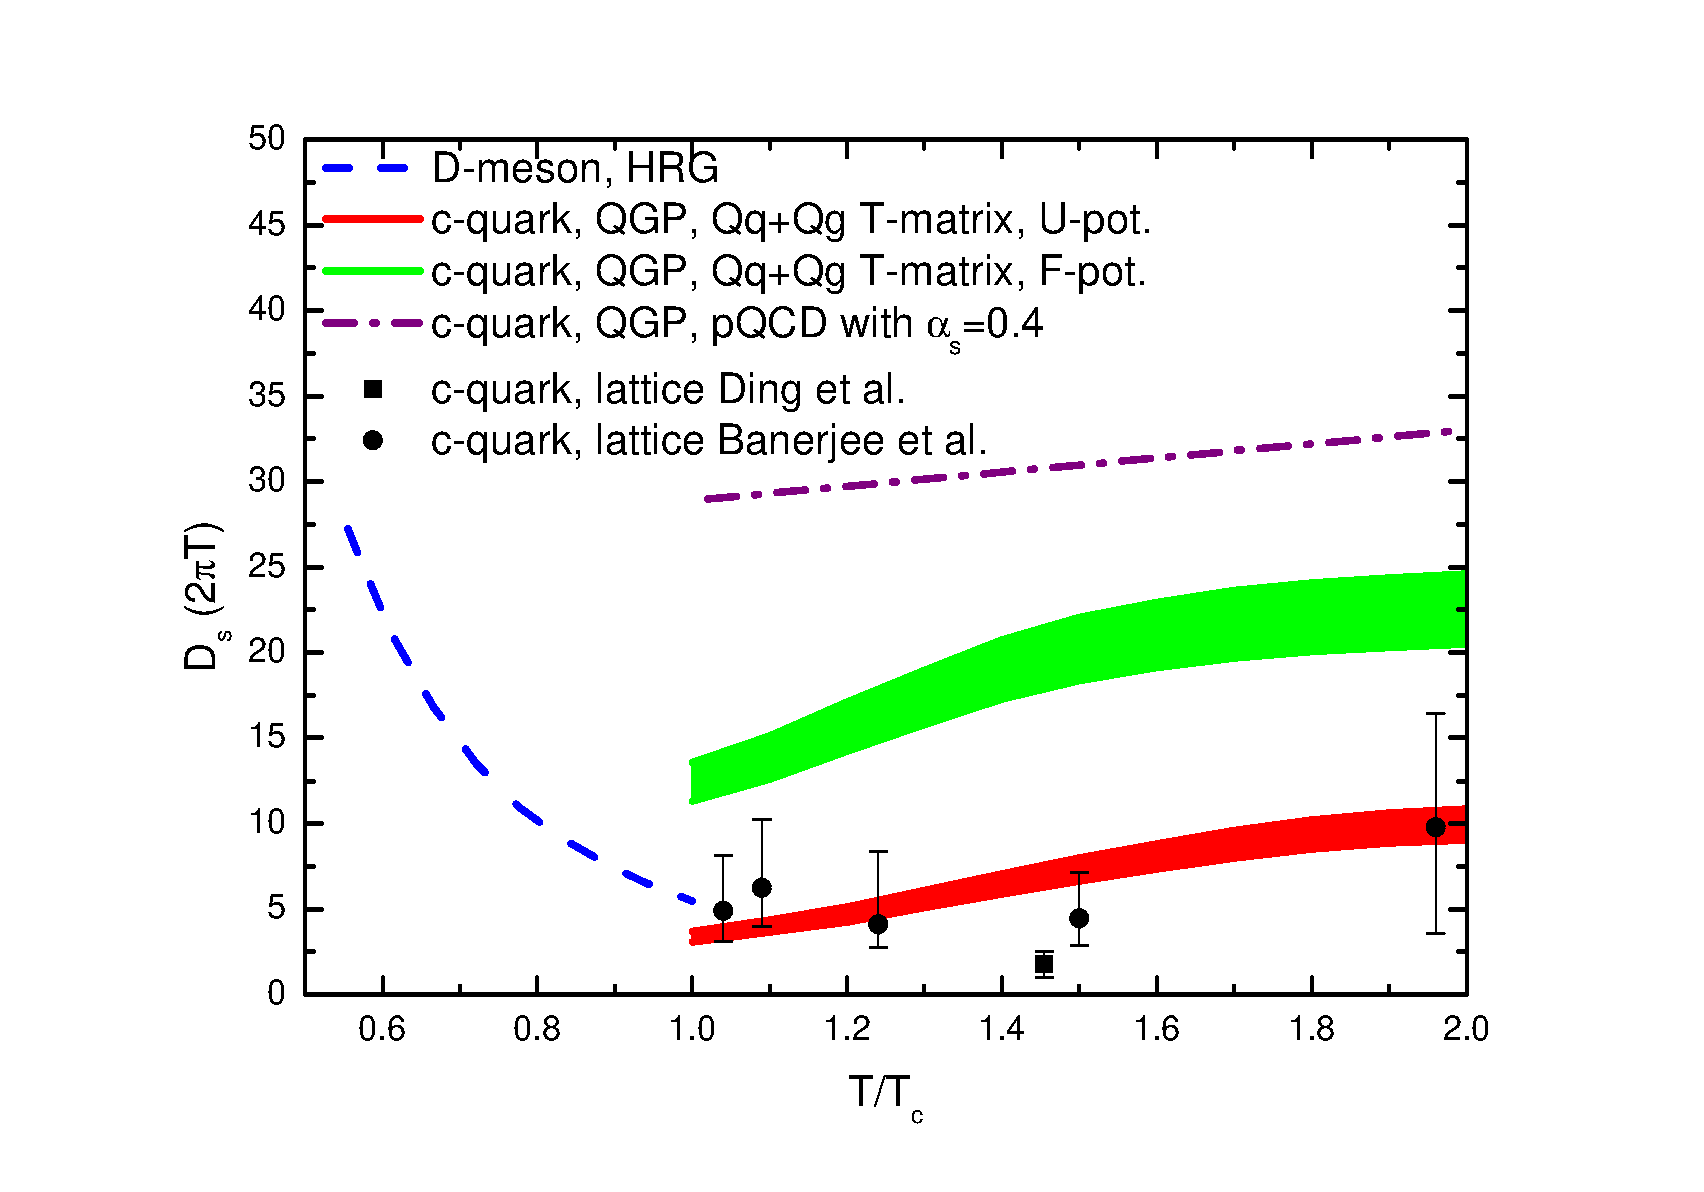
\includegraphics[width=1.00\textwidth]{fig/Ds-2piT} }
 \caption[Spatial diffusion coefficient for charm quarks and $D$-mesons]{Spatial diffusion coefficient for charm quarks in the QGP ($T>T_{\rm c}$)
 and $D$-mesons in hadronic matter ($T<T_{\rm c}$), in units of the thermal wavelength.
 The data points are extracted from quenched 
 lattice QCD~\cite{Banerjee:2011ra,Ding:2012sp,Kaczmarek:2014jga} while the bands are 
 obtained from potential-based $T$-matrix calculations~\cite{Riek:2010fk,Huggins:2012dj} 
 using either the free (green) or internal (red) energies from lattice QCD. The dash-dotted 
 line corresponds to leading order perturbation theory~\cite{Svetitsky:1987gq}.
 }
 \label{fig:Ds-2piT}
 \end{figure}
 Progress has been made to extract $D_s$ from first principles in thermal lattice QCD, 
 by computing euclidean heavy-quark (HQ) correlation functions and reconstructing the 
 low-energy limit of the pertinent spectral function (which defines the transport coefficient). 
 Thus far this has been done in quenched QCD (i.e., in a gluon plasma without dynamical 
 quarks)~\cite{Banerjee:2011ra,Ding:2012sp,Kaczmarek:2014jga}, resulting in a range of 
 values of $D_s(2\pi T) \simeq$~2-6 for temperatures between 1-2~$T_c$, as shown in 
 Figure~\ref{fig:Ds-2piT}. 
 To make closer contact to experiment, it will be necessary to extend these studies 
 to QCD with dynamical quarks, and to compute the 3-momentum dependence of the transport 
 coefficient. The latter can be alternatively expressed through the thermal relaxation 
 rate, $\gamma_Q=T/(m_Q D_s)$, where $m_Q$ is the HQ mass in the QGP, or heavy-meson mass 
 in hadronic matter. 
 
 Non-perturbative calculations of the HQ transport coefficients have also been carried out 
 in the thermodynamic $T$-matrix formalism~\cite{vanHees:2007me,Riek:2010fk,Huggins:2012dj}, 
 which is based on a potential approximation for HQ scattering off thermal partons. The 
 in-medium potential can, in principle, be extracted from thermal lattice QCD, see, e.g., 
 Ref.~\cite{Burnier:2014ssa}. Current uncertainties are usually bracketed by employing 
 either the HQ internal or free energies from the lattice. Using the internal energy one 
 finds values of $D_s(2\pi T)\simeq$\,3-5 at temperatures close to $T_{\rm c}$, increasing 
 to about 10 at 2\,$T_{\rm c}$, for both charm and bottom quarks, see Figure~\ref{fig:Ds-2piT}. 
 For the free energy, the $D_s$ values are about a factor of 2-4 larger. The relaxation 
 rates from the $T$-matrix formalism predict an appreciable 3-momentum dependence, decreasing 
 toward perturbative values at high momenta. Close to $T_{\rm c}$, resonant structures develop 
 in the heavy-light quark $T$-matrices, suggestive of the onset of hadronization. 
 
 Recent work has demonstrated the importance of also treating the  $D$ meson diffusion in the hadronic 
 phase. The pertinent transport coefficient has been estimated 
 in heavy-meson chiral perturbation theory~\cite{Laine:2011is} and in effective 
 hadronic theories including resonance 
 scattering~\cite{He:2011yi,Ghosh:2011bw,Abreu:2011ic,Tolos:2013kva}. The $D$-meson 
 diffusion coefficient significantly decreases as $T_{\rm c}$ is approached from below. 
 There is increasing consensus that its hadronic values~\cite{He:2011yi,Tolos:2013kva} 
 come close to the nonperturbative approaches on the QGP side. This suggests that the 
 heavy-flavor diffusion coefficient develops a minimum across the phase transition 
 region, with a near-continuous temperature dependence when passing from hadronic 
 to partonic degrees of freedom, as one would expect in a cross-over 
 transition~\cite{He:2011yi,He:2012df,Tolos:2013kva}. 
 
 \begin{figure}[tbh] 
 \centerline{ \includegraphics[width=0.90\textwidth]{fig/D-RAA-star} } 
 \caption[STAR measurements of $D$-meson production compared to theory]{Nuclear modification factor of $D$-mesons in 200 GeV \AuAu\ collisions 
 at various centralities as measured by STAR~\cite{Adamczyk:2014uip}, compared to 
 theoretical 
 calculations~\cite{Adil:2006ra,Gossiaux:2008jv,He:2011qa,Alberico:2013bza,Cao:2013ita} 
 } 
 \label{fig:D-RAA-star} 
 \end{figure} 
 Remarkable results for open heavy-flavor observables have recently been obtained at 
 both RHIC and the LHC. The STAR~\cite{Adamczyk:2014uip} and 
 ALICE~\cite{Alice:2012ab,Abelev:2013lca,Abelev:2014ipa} collaborations have, for the 
 first time, been able to extract the nuclear modification factor ($R_{AA}$) and 
 elliptic flow ($v_2$) of $D$ mesons. The STAR measurement of $D$ mesons in 200 GeV 
 Au-Au reaches down to rather low transverse momenta ($p_T$)~\cite{Adamczyk:2014uip}, 
 showing intriguing evidence for a maximum in the $R_{AA}(p_T)$ as seen in 
 Figure~\ref{fig:D-RAA-star}. Such a structure is a tell-tale signature for collective 
 behavior of $D$ mesons, which in turn requires a strong coupling of $c$ quarks and $D$ mesons 
 to the expanding medium. As part of the thermalization process, the heavy-flavor
 particles are dragged along in the fireball expansion and accumulate in a momentum range
 characteristic of the medium's collective flow velocity, while low- and high-momentum states are 
 depleted. This feature can be described by theoretical calculations which implement 
 (a) a sufficiently small diffusion coefficient of $ D_s (2\pi T) \leq5$ into dynamical 
 evolution models~\cite{He:2011qa,Gossiaux:2008jv,Cao:2013ita}, and 
 (b) heavy-light 
 quark coalescence in the hadronization process. The precise location of the
 flow bump turns out to be rather sensitive to the underlying bulk evolution model. 
 Systematic comparisons of the different ingredients to the theoretical models and 
 improved precision in the data are required to disentangle the different effects and 
 arrive at quantitative results for the heavy-quark transport coefficient. 
 Additionally, measurements of the $R_{AA}$ of $D_s$ mesons (containing one charm and 
 one strange anti-/quark), would be very helpful as coalescence processes of $c$ quarks 
 with the enhanced strangeness content of the QGP significantly augment the flow 
 bump~\cite{He:2012df}.  

 A critical role in the determination of the transport coefficient is played by measurements of the elliptic flow parameter
 $v_2$ of the heavy-flavor particles. Electrons and muons from semileptonic decays 
 of $D$- and $B$-meson have been found to carry a rather large $v_2$ in heavy ion
 collisions at both RHIC~\cite{Adare:2006nq,Mustafa:2012jh} and the LHC~\cite{Sakai:2013ata}. 
 Important midterm goals at RHIC are to disentangle the $B$ and $D$ contributions to the semileptonic decays, and to 
 obtain an independent measurement of the $v_2$ of directly reconstructed $D$ mesons. 
 The former will be extracted from existing RHIC 2014 Au+Au displaced vertex 
 measurements by PHENIX (using the VTX and FVTX detectors)~\cite{Nouicer:2012pr}, and by 
 STAR (using the HFT detector)~\cite{Kapitan:2008kk,Qiu:2014dha}. The $v_2$ of directly reconstructed $D$ mesons 
 will be obtained from the same data set using the STAR HFT~\cite{Qiu:2014dha}. 
 At the LHC, ALICE has 
 conducted first measurements of the $D$-meson $v_2$ in 2.76\,TeV \PbPb\ 
 collisions~\cite{Abelev:2013lca}, and found large values; CMS has been able to extract 
 a $B$-meson $R_{AA}$ through their displaced-vertex decays into $J/\psi$'s (so-called 
 non-prompt $J/\psi$'s~\cite{Chatrchyan:2012np}, which is approximately unity for small  
 momenta and turns into a suppression leveling off at $\sim$0.5 at high momenta. As 
 in the $D$-meson sector, this is consistent with collective behavior and thus indicative 
 for a strong bottom coupling to the medium, providing further valuable model constraints.

 An outstanding  issue is the determination of the temperature dependence of the transport coefficient.  
 Experimentally, one lever arm is provided by the correlation between $v_2$ and the 
 $R_{AA}$. Since the bulk medium $v_2$ takes several fm/$c$ to build up, a large $v_2$ 
 of the HF particles is indicative for a strong coupling in the later QGP phases of the 
 fireball evolution, and through hadronization. 
 A suppression in the $R_{AA}$, on the other hand, begins immediately in the early 
 high-density phases, especially at high $p_T$. Model calculations to date
 cannot easily account for the large $D$-meson $v_2$ at LHC without overestimating 
 the suppression in the $R_{AA}$. This corroborates a strong coupling in the vicinity
 of $T_{\rm c}$. The second lever arm is provided by going to lower collision 
 energies where the system starts out at smaller QGP temperatures, closer to $T_{\rm c}$. 
 First data for the heavy-flavor electron $R_{AA}$ and $v_2$ have been extracted
 from a 62\,GeV run at RHIC~\cite{Adare:2014rly,Adamczyk:2014yew}, and show evidence 
 for a non-vanishing $v_2$ and marked modifications in the $R_{AA}$. They are not 
 imcompatible with model calculations that utilize a strong heavy-flavor coupling around 
 $T_c$~\cite{He:2014epa}, but the data precision does not yet suffice for clear conclusions. 
 While varying the collision energy is a valuable tool to explore the temperature 
 dependence of these phenomena, it is necessary to account for the 
 more pronounced role of the Cronin effect at these energies, i.e., 
 a modification of the heavy-flavor spectra through cold nuclear matter effects, before 
 the QGP forms. 
Here  \pA\ collisions will be important to quantify these effects in order to provide a realistic starting 
point for assessing the hot-medium effects. 
 
  

%\bibliographystyle{atlasnote}
%\bibliography{OpenHeavyFlavor}

%\end{document}




\subsection{Thermal Radiation and Low-Mass Dileptons}
        \label{Sec:EM}

Electromagnetic (EM) radiation from the fireballs created in heavy-ion collisions
has long been recognized as a valuable probe of hot and dense
matter~\cite{Feinberg:1976ua,Shuryak:1978ij}. Once produced, photons and dileptons
traverse the fireball and reach the detectors without further
re-interaction. Therefore, their measured spectra are direct signals from the hot and dense
phases of the fireball. In particular, thermal radiation from the locally equilibrated
matter contains unique information about the QCD medium.

The physics potential of EM radiation can be gleaned from the expression for its
local emission rate. At a temperature $T$ it is given by
\begin{equation}
R_{\rm EM} = {\rm const} \ f(E;T) \ \rho_{\rm EM}(M,p;T)
\label{eq:rate}
\end{equation}
where $f(E;T)\simeq \exp(-E/T)$ is the thermal distribution function and
$\rho_{\rm EM}(M,p;T)$ the EM spectral function; $M$ is the invariant mass of the
dilepton ($M$=0 for photons), $p$ its 3-momentum and $E=\sqrt{M^2+p^2}$ its energy.
The mass dependence of $\rho_{\rm EM}$ reflects the operational degrees of freedom:
in vacuum, the low-mass region ($M\le 1$~GeV) is saturated by the light vector mesons
$\rho$, $\omega$ and $\phi$, while the intermediate-mass region (1.5~$\le M/\GeV \le$~3)
is characterized by a perturbative quark-anti-quark continuum.

Calculations of thermal dilepton and photon spectra suitable for comparison to
experiment require the emission rate, Eq.~(\ref{eq:rate}), to be integrated over a
realistic space-time evolution of the fireball in heavy-ion collisions, e.g., by
using hydrodynamic models. The following properties of the QCD medium can then be
studied with EM emission spectra in heavy-ion collisions.
\begin{description}
\item[In-Medium Properties of Vector Mesons.]
In the low-mass region, dilepton radiation from the fireball monitors the
medium effects on the vector mesons as the QCD phase transition is approached and
surpassed. In the vacuum, the properties of light hadrons are governed by the
spontaneously broken chiral symmetry induced by the formation of a quark-anti-quark
condensate. The reduction of the condensate in the QCD medium~\cite{Borsanyi:2010bp}
therefore imposes marked changes on the hadron spectrum. Low-mass dileptons are a
unique observable to measure these modifications in the vector meson mass spectrum.
\item[Temperature of the Fireball.]
Dilepton spectra in the intermediate-mass region\linebreak
($1.5 \le M/\GeV \le 3$) provide a
pristine thermometer of the fireball. Since the medium modifications of the continuum
in the EM spectral function, $\rho_{\rm EM}$, are small (suppressed by the ratio
$T^2/M^2$), the spectral slope of the radiation is solely determined by the temperature
in the thermal distribution function, $f(E;T)\simeq{\rm e}^{-E/T}$. For large masses,
its exponential form strongly favors radiation from the hottest phases of the
fireball~\cite{Shuryak:1980tp,Rapp:2004zh}, so that the observed spectra are mostly
emitted from early in the evolution. Since the mass spectra are
Lorentz-{\em invariant}, they are not distorted by a Doppler shift
from the collective expansion of the exploding fireball.
\item[Lifetime of the Fireball.]
The total yields of thermal EM radiation are a measure of the total lifetime of the
emitting fireball (the expanding 3-volume is constrained by final-state hadron yields).
The optimal mass window for this measurement appears to be
$M\simeq$\,0.3-0.7\,GeV~\cite{Rapp:2014hha}, where the radiation yields turn out to
be proportional to the fireball lifetime within about 10\%,
over a large range of heavy-ion collision energies~\cite{Rapp:2014hha}.
\item[Collective Properties of the Emission Source.]
In contrast to the invariant-mass spectra, the transverse-momentum spectra of dileptons
and photons are subject to a Doppler shift: the expansion velocity of the medium
imparts additional energy on the photons and dileptons which makes their spectra appear
``hotter". The slope of the transverse-momentum spectra is therefore determined by both
the temperature and collective-flow properties of the emitting source.
Another powerful observable is the elliptic flow of the EM radiation. Since the elliptic
flow of the bulk medium takes several fm/c to build up, the elliptic flow of the EM
radiation further constrains the origin of its emission.
\end{description}

The physics potential of accurate dilepton data has been demonstrated by the NA60
collaboration at the CERN SPS in collisions of medium-sized nuclei (Indium with A=114)
at an energy of
$\sqrt{s_{NN}}$=17.3\,GeV~\cite{Arnaldi:2008fw,Arnaldi:2008er,Specht:2010xu}. The
low-mass spectra confirmed the gradual melting of the $\rho$-meson resonance into a
structureless quark-anti-quark continuum, while the total yields translate into an
average fireball lifetime of $7\pm1$\,fm/c. The inverse slope of the radiation at
intermediate masses gives an average temperature of $205\pm12$\,MeV, signaling QGP
radiation. The radial-flow pattern in the transverse-momentum spectra confirms
predominantly hadronic and QGP sources at low and intermediate masses, respectively.
Broad dilepton measurements at different energies with heavy projectiles are needed
to exploit this potential for systematic studies across the QCD phase diagram.

\begin{figure}[tbh]
\centerline{
\includegraphics[width=0.45\textwidth]{fig/dNeedM-star}
\includegraphics[width=0.55\textwidth]{fig/excessLMRTheoryComp_tau1}
}
\caption[STAR Beam Energy Scan results on di-electron yields]{Di-electron invariant-mass spectra as measured by
STAR~\cite{Adamczyk:2013caa,Huck:2014mfa} in \AuAu\ collisions in the first beam
energy scan at RHIC. The left panel shows the invariant-mass spectra for increasing
collision energies (bottom to top); the orange bands represent the sum of theoretically
predicted thermal radiation~\cite{Rapp:2013nxa} from QGP and hadronic matter
and final-state hadron decays (including their uncertainty). At intermediate masses
($M>1$\,GeV) the spectra are dominated by correlated heavy-flavor decays and are not yet
sensitive to thermal radiation. 
%The right panel shows the dielectron
%transverse pair momentum spectra in the low mass range, $0.4<M/\GeV<0.76)$, again compared
%to the sum (solid line) of thermal radiation and final-state hadron decays.
The right panel shows integrated yields of the normalized dilepton excesses 
for $0.4<M_{ll}<0.75$ GeV/$c^{2}$ as a function of $dN_{\rm ch}/dy$~\cite{Adamczyk:2015bha,Specht:2010xu}. 
The theoretical lifetimes inferred from a model calculation~\cite{Rapp:2014hha} are also shown
}
\label{fig:star-ee}
\end{figure}
A first step in this direction has recently been made by
STAR~\cite{Adamczyk:2013caa,Huck:2014mfa,Adamczyk:2015bha} in the BES program at RHIC. In \AuAu\
collisions covering energies from SPS to top RHIC ($\sqrt{s_{NN}}$=19.6, 27, 39, 62, 200\,GeV),
a sustained low-mass excess radiation was found, cf.~Figure~\ref{fig:star-ee}.
Both mass and transverse-momentum spectra are well described by thermal radiation from
hadronic matter and QGP~\cite{Rapp:2013nxa} (added to contributions from final-state
hadron decays). The data corroborate the melting of the $\rho$  as a robust mechanism of the low-mass
excess in the hadron-to-quark transition at small and moderate baryon chemical potential.
Improved measurements of the low-mass spectral shape at small chemical
potential~\cite{Adamczyk:2013caa} will be critical to discriminate theoretical
models~\cite{Rapp:2000pe,Dusling:2007su,Linnyk:2011vx,Xu:2011tz,Vujanovic:2013jpa}.
This is expected from upcoming high-luminosity \AuAu\ running at 200\,GeV. Lifetime
``measurements" via the integrated low-mass excess require less precision. 
Comparison of 
the BES-I data at $\sqrt{s_{NN}} = $ 19.6 and 200 GeV to theoretical models indicate
that the normalized excess dilepton yields in the low mass region are proportional to the calculated lifetimes of the medium, 
as shown in the right panel of Figure~\ref{fig:star-ee}.
These measurements can be performed with much improved precision in the upcoming BES-II campaign, 
providing a tool to
detect lifetime ``anomalies" possibly induced in the vicinity of a critical
point~\cite{Rapp:2014hha}.

Theoretical progress has been made in elaborating the connection of the dilepton data
to chiral symmetry restoration~\cite{Hohler:2013eba}. The broadening $\rho$-meson
spectral function used to describe the dilepton spectra has been tested  with Weinberg
and QCD sum rules which relate vector and axial-vector spectral functions to quark and
gluon condensates. With temperature-dependent condensates taken from
lattice QCD~\cite{Borsanyi:2010bp}, solutions for the axial-vector spectral function
were found which accurately satisfy the in-medium sum rules. Thus the melting of the
$\rho$-meson resonance is compatible with (the approach to) chiral symmetry restoration.
Further progress has been made in evaluating the in-medium vector correlation function,
and the associated thermal dilepton rates, in thermal lattice
QCD~\cite{Ding:2010ga,Brandt:2012jc}. The computed correlation functions in the QGP
encode a low-mass enhancement which is quite compatible with the spectral functions
that figure into the explanation of the observed dilepton spectra~\cite{Rapp:2011is}.

\begin{figure}[tbh]
\centerline{\includegraphics[width=1.0\textwidth]{fig/gam-spec-v2-phenix} }
\caption[PHENIX results on direct photon spectra and flow compared to theory]{Direct photon spectra (left panel) and their elliptic flow (right panel) in 0-20\%
\AuAu\ collisions at 200\,GeV energy. PHENIX data~\cite{Adare:2011zr,Adare:2014fwh,Bannier:2014bja}
are compared to theoretical model calculations~\cite{vanHees:2011vb,Shen:2013cca,Linnyk:2013wma}.
}
\label{fig:phenix-gam}
\end{figure}
An excess signal of low-momentum direct photons, beyond expectations from binary
nucleon-nucleon collisions and final-state hadron decays, has been measured by
PHENIX~\cite{Adare:2008ab} in 200\,GeV \AuAu\ collisions. The transverse momentum spectra of 
the excess photons are of exponential shape with an inverse slope parameter 
$T_{\rm slope}\simeq 240\pm 30$\,MeV~\cite{Adare:2008ab,Adare:2014fwh}.
As noted above, Doppler shifts due to the collective medium expansion need to be accounted for
in extracting the temperature. Theoretical models suggest that the emission mainly originates
from the later QGP and hadronic stages of the fireball, from a rather broad window of
temperatures around $T_{\rm pc}\simeq170$\,MeV, with an average medium expansion velocity of
$\sim$0.3-0.5$c$~\cite{vanHees:2011vb,Shen:2013cca}. The experimental yields tend to be
underestimated by currently available calculations for thermal radiation, as shown in the left
panel of Figure~\ref{fig:phenix-gam}. Similar measurements are also becoming available
from STAR~\cite{Yang:2014mla}.

The direct photon excess carries a surprisingly large elliptic flow
($v_2$)~\cite{Adare:2011zr,Bannier:2014bja} as seen in the right panel of Figure~\ref{fig:phenix-gam}.
In fact, the magnitude of the flow is comparable to that of pions, which are emitted
when the fireball decouples. This is incompatible with
a large contribution to the direct photon excess from early QGP
radiation~\cite{Chatterjee:2005de,Liu:2009kta,Holopainen:2011pd,vanHees:2011vb,Dion:2011pp,Shen:2013cca,Linnyk:2013wma},
and again points to a later emission of the excess photons. The elliptic flow strength $v_2$ also is underestimated
by current theoretical calculations, but more precise data are needed to quantify the discrepancies.

The PHENIX data have triggered substantial theoretical activity. To obtain sufficiently large yields 
{\em and} a large $v_2$ from a thermal photon source the bulk medium would need to develop its final $v_2$ rather 
rapidly, probably before reaching the phase transition regime~\cite{vanHees:2011vb}. This could be driven, 
e.g., by a pre-equilibrium radial flow from a glasma evolution~\cite{Dusling:2010rm,Chen:2013ksa}.
Such favorable collective properties would also need to be accompanied by large photon rates in the phase transition
regime~\cite{vanHees:2011vb,Shen:2013vja,vanHees:2014ida} and in the hadronic
phase~\cite{Turbide:2003si}. An initially gluon-rich plasma~\cite{McLerran:2014hza}, or 
nonperturbative effects in a QGP~\cite{Gale:2014dfa}, could aid in suppressing
early electromagnetic emission when the bulk $v_2$ is still small
and thereby avoid diluting the observed strong $v_2$ pattern with the azimuthally symmetric
distribution expected for photons emitted early in the collision.

Preliminary measurements of the direct-photon triangular flow ($v_3$)~\cite{Bannier:2014bja}
support a thermal emission source~\cite{Shen:2013cca} and disfavor more exotic sources, e.g.,
from strong but short-lived primordial magnetic fields~\cite{Basar:2012bp,Bzdak:2012fr}.
The centrality dependence of the excess signal~\cite{Adare:2014fwh} is consistent
with expectations from thermal radiation, but is also compatible with scaling arguments based on
initial-state saturation effects~\cite{McLerran:2014oea}. Improved measurements of the
photon spectra and their collective properties will be critical in resolving these issues, as will 
be extending these measurements to other colliding systems. 

Closely related but independent observables are the transverse-momentum spectra and $v_2$ of
low-mass dileptons.
A first measurement of
the $v_2$ has been achieved~\cite{Adamczyk:2014lpa} but does not yet provide tangible
discrimination power. 
Again, improved and extended experimental measurements are required, as well
as additional calculations. Since photons and dileptons are intimately related in theoretical
calculations, a complete understanding of EM data and its implications for the thermal 
history of the medium will need to account for both observables
simultaneously.


\subsection{Mapping the Phase Diagram of QCD via a Beam Energy Scan}
\label{Sec:BES}




When the first protons and neutrons and pions formed in the
microseconds-old universe, and when they form in heavy-ion collisions
at the highest RHIC energies and at the LHC, they condense out of
liquid quark-gluon plasma consisting of almost as much antimatter as
matter. Lattice calculations~\cite{Aoki:2006we,Aoki:2009sc,Bazavov:2011nk} 
show that QCD predicts that, in such an environment, this condensation 
occurs smoothly as a function of decreasing temperature, with many 
thermodynamic properties changing dramatically but continuously within 
a narrow temperature range around the transition temperature 
$T_c\in [145\,\mathrm{MeV},163\,\mathrm{MeV}]$
\cite{Bazavov:2011nk,Bazavov:2014pvz}, referred to as the crossover
region of the phase diagram of QCD, see Figure~\ref{F-PD1}.
%
\begin{figure}[t]
\begin{center}
\centerline{\includegraphics[width=0.65\textwidth]{fig/Phasediagram.png}}
\caption[The QCD phase diagram]{A sketch illustrating the experimental and theoretical
  exploration of the QCD phase diagram. Although experiments at
  highest energies and smallest baryon chemical potential are known to
  change from a QGP phase to a hadron gas phase through a smooth
  crossover, lower energy collisions can access higher baryon chemical
  potentials where a first order phase transition line is thought to
  exist.}
\label{F-PD1}
\end{center}
\end{figure}
%%%%%%%%%%%%%%%%%%%%% Figure PD-1 %%%%%%%%%%%%%%%%%%%%%%%%%%%%%%%%%%%%%%%%%%%%%%%
%\begin{figure}[htb]
%\begin{center}
%\begin{minipage}{0.6\textwidth}
%\includegraphics[width=\textwidth]{fig/Phasediagram.png}
%\end{minipage}
%\hspace*{4mm}
%\begin{minipage}{0.35\textwidth}
%\caption{A sketch illustrating the experimental and theoretical
%  exploration of the QCD phase diagram. Although experiments at
%  highest energies and smallest baryon chemical potential are known to
%  cross from a QGP phase to a hadron gas phase through a smooth
%  crossover, lower energy collisions can access higher baryon chemical
%  potentials where a first order phase transition line is thought to
%  exist.
%\label{F-PD1}
%}
%\end{minipage}
%\end{center}
%\end{figure}
%%%%%%%%%%%%%%%%%%%%%%%%%%%%%%%%%%%%%%%%%%%%%%%%%%%%%%%%%%%%%%%%%%%%%%%%%%%
%
In contrast, quark-gluon plasma doped with a sufficient excess of
quarks over anti-quarks may instead experience a sharp first order
phase transition as it cools, with bubbles of quark-gluon plasma and
bubbles of hadrons coexisting at a well-defined critical temperature,
much as bubbles of steam and liquid water coexist in a boiling
pot. The point where the doping of matter over antimatter
(parametrized by the net baryon number chemical potential $\mu_B$)
becomes large enough to instigate a first order phase transition is
referred to as the QCD critical point. It is not yet known whether QCD
has a critical point~\cite{Stephanov:1998dy,Fodor:2004nz,Allton:2005gk,Gavai:2008zr,deForcrand:2008zi},
nor where in its phase diagram it might lie. Lattice calculations
become more difficult or more indirect or both with increasing $\mu_B$
and, although new methods introduced within the past decade have
provided some hints~\cite{Fodor:2004nz,Gavai:2008zr,Datta:2012pj}.
While these theoretical calculations are advancing through both
new techniques and advances in computational power,
at present only experimental measurements can answer these questions
definitively. 


The phase diagram of QCD, with our current knowledge shown schematically
in Figure~\ref{F-PD1}, is the only phase diagram of any form of
matter in Nature that we have the opportunity of both mapping experimentally
and relating directly and quantitatively to our fundamental
description of Nature, the Standard Model. With QCD the only strongly
interacting theory in the Standard Model, mapping the transition
region of its phase diagram is a scientific goal of the highest
order. In the long term, successfully connecting a quantitative,
empirical understanding of its phases and the transitions between
phases to theoretical predictions obtained from the QCD Lagrangian
could have ramifications in how we understand phases of strongly
coupled matter in many other contexts.

%%%%%%%%%%%%%%%%%%%%%%%%%%%%%%%%%
{\bf RHIC's unique capability to probe the QCD phase diagram}
%%%%%%%%%%%%%%%%%%%%%%%%%%%%%%%%%

A major effort to use heavy ion collisions at RHIC to survey the phase
diagram of QCD is now underway. The excess of matter over antimatter
in the exploding droplet produced in a heavy ion collision can be
increased by decreasing the collision energy, which reduces the
production of matter-antimatter symmetric quark-antiquark pairs and
gluons relative to the quarks brought in by the colliding nuclei, thus
increasing $\mu_B$. Decreasing the collision energy also decreases the
maximum, {\it i.e.}~initial, temperature reached by the matter produced in
the collision. A series of heavy ion collision measurements scanning
the collision energy~\cite{BESII} can therefore explore the properties
of matter in the crossover region of the phase diagram, matter that is
neither quark-gluon plasma nor hadronic nor both at the same time, as a
function of the doping $\mu_B$. Such a program can scan the transition
region of the QCD phase diagram out to $\mu_B$ values that correspond
to collision energies below which the initial temperature no longer
reaches the transition. If the crossover region narrows to a critical
point within this experimentally accessible domain, an energy scan can
find it. RHIC completed the first phase of such an energy scan in
2014, taking data at a series of energies ($\sqrt{s_{NN}}=$ 200, 62.4,
39, 27, 19.6, 14.5, 11.5 and 7.7 GeV) corresponding to values of
$\mu_B$ that range from 20 to 400 MeV. Data from these experiments at
RHIC~\cite{Kumar:2012fb,BESII} and from previous experiments confirm that
lower-energy collisions produce matter with higher $\mu_B$, as
anticipated. 

RHIC is, and will remain, the optimal facility in the world for
mapping the phase diagram of QCD, including searching for a possible
critical point in its so far less well understood regions with larger $\mu_B$.
%studying matter in the crossover region and searching for a possible
%critical point in the so far less well understood regions of the phase
%diagram with larger $\mu_B$. 
What makes RHIC unique is both its wide
reach in $\mu_B$ and that it is a collider, meaning that the
acceptance of detectors, and hence the systematics of making
measurements, change little as a function of collision
energy. Accelerator and detector performance has been outstanding
during the first phase of this program, referred to as Beam Energy
Scan I or BES-I. Measurements of all the important observables
targeted in the planning of this campaign have now been made in
collisions with energies varying by a factor of 25, allowing for a
first look at a large region of the phase diagram of QCD.

A selection of measurements of several observables from BES-I that exhibit interesting 
non-monotonic behavior as a function of collision energy is shown in 
Section~\ref{Sec:CP}, see Figure~\ref{F-PD2} there.  
As we will discuss in that later section, the BES-I measurements of these 
observables provide some
evidence for the softening of the equation of state in the 
crossover region of the phase diagram. 
In addition, these data may indicate
the first hints of the presence of a critical point in the phase
diagram of QCD. Above all, given the size of the present
experimental uncertainties these current measurements 
provide strong motivation
for the next phase of the BES program BES-II, described in Section~\ref{Sec:CP}, which will deliver in 2018-19
substantially greater statistics and hence substantially smaller error bars
in collisions with energies at and below $\sqrt{s_{NN}}$=19.6 GeV.
Accordingly, we defer our presentation of  highlights from the rich BES-I data set to 
Section~\ref{Sec:CP}
where we will discuss each observable in a way that synthesizes
what we have learned from data to date with what can be learned
from their measurement in BES-II in combination with anticipated advances
in theory.





\subsection{Topological Fluctuations within Quark-Gluon Plasma}
\label{Sec:Exotica}

It has been known for decades that topological effects play an
important role in determining the structure of the vacuum in
non-Abelian gauge theories\cite{Belavin:1975fg}.  In QCD, fluctuations
that change the topology of the non-Abelian gauge fields are at the
same time fluctuations that create an imbalance of chirality.
Recently, considerable interest has been generated by the possibility
of exploring experimental signatures of such fluctuations in the hot
QCD matter produced in relativistic heavy ion collisions.  A key
observation is that the incredibly strong magnetic field that is
generated in off-center heavy ion collisions, together with the chiral
anomaly in QCD and the fluctuations in chirality, can produce a Chiral
Magnetic
Effect~\cite{Kharzeev:2007tn,Kharzeev:2007jp,Fukushima:2008xe,Hirono:2014oda}
in which an electric current flows along (for one sign of the
chirality fluctuation) or opposite to (for the other sign of the
chirality fluctuation) the direction of the magnetic field, resulting
in a separation of particles with opposite electric charge in a
direction perpendicular to the reaction plane of the collision, while
particles with the same electric charge show a preference for ending
up in the same hemisphere.
\begin{figure}[!htp]
\includegraphics[width=\textwidth]{fig/CMEfromBES.pdf}
\caption[Charge separation results from STAR and ALICE]{Collision energy dependence of the charge separation
  correlation $H$ difference between same-sign (SS) and opposite sign
  (OS) pairs in mid-central (30-60\%) \AuAu\ collisions by RHIC\cite{Adamczyk:2014mzf}
  ($\sqrt{s_{NN}}= 7.7 - 200$ GeV) and Pb+Pb collisions at LHC\cite{Abelev:2012pa}
  ($\sqrt{s_{NN}}= 2.76$~TeV). The hatched band represents the
  estimated statistical errors that will be obtained in BES II
  measurements at RHIC.}
\label{Fig:CME}
\end{figure}

Such an effect has been observed by using the three-point correlator
method~\cite{Voloshin:2004vk} to extract event-plane dependent charge
correlations in \PbPb\ collisions at the LHC~\cite{Abelev:2012pa} and
at a variety of collision energies at
RHIC\cite{Abelev:2009ac,Abelev:2009ad,Adamczyk:2014mzf}.  Conclusively
establishing that these observations result from the CME would be an
important advance in our ability to study experimentally the
topological phase structure of QCD.  In addition, the effect itself
can be used to study the properties of the medium created in the
collisions. Since the CME requires the formation of QGP, {\it e.g.}
the restoration of the chiral symmetry~\cite{Hirono:2014oda}, one
would expect that at sufficiently low energy, the QCD related
correlations should disappear. This is precisely what is observed in
$\sqrt{s_{NN}}$=11.5 GeV \AuAu\ collisions~\cite{Adamczyk:2014mzf}, as
shown in Figure~\ref{Fig:CME}.

\begin{figure}[!htp]
\includegraphics*[width=0.9\textwidth]{fig/CVEfromSTAR}
\vspace{-1.5cm}
\caption[Baryon separation as a function of collision centrality from STAR]{Baryon separation shown as a function of collision centrality
  from $\sqrt{s_{NN}}=200$ GeV Au+Au collisions. Circles and triangles
  represent the data for the same-baryon-number and
  opposite-baryon-number correlations, respectively.  Error bars are
  statistical only. Taken from \cite{Zhao:2014aja}.}
\label{Fig:CVE}
\end{figure}
The same physical mechanism that produces the Chiral Magnetic Effect
in the presence of a magnetic field $\vec B$ can also produce a Chiral
Vortical Effect (CVE) in the presence of external angular momentum
$\vec L$~\cite{Kharzeev:2010gr}.  While high energy nuclear collisions
produce the strongest known magnetic fields $\sim 10^{18}$
gauss\footnote{The magnetic field at the surface of magnetars is on
  the order of $10^{15}$ gauss, several orders of magnitude lower than
  the field strength in high-energy nuclear collisions.}, these fields
are largest at the very beginning of the collision and decay away on a
timescale that is controlled by the electric conductivity of the
matter produced in the
collision~\cite{Tuchin:2013ie,McLerran:2013hla,Gursoy:2014aka}.
Angular momentum, on the other hand, is conserved meaning that if the
plasma is created with nonzero angular momentum this remains.  If
topological fluctuations and the associated chirality fluctuations do
have observable effects in high energy nuclear collisions, then in
addition to the charge separation along the external magnetic field in
the CME one would expect baryon number separation along the (same)
direction of the external angular momentum.  The first measurements of
observables that receive a contribution from any CVE were reported
recently for \AuAu\ collisions at 200 GeV for proton (anti-proton) and
Lambda (anti-Lambda) pairs~\cite{Zhao:2014aja}, as shown in
Figure~\ref{Fig:CVE}.  The figure indicates a preference for proton
and Lambda pairs, as well as antiproton and anti-Lambda pairs, to be
found in the same hemisphere.

%Both the CME or CVE are consequences of the fundamental symmetries of QCD. 
%Therefore the underlying physics is not limited to high energy nuclear collisions, but should be expected in other strongly interacting systems.

The topological fluctuations that drive the CME and CVE in QCD have
analogues in other gauge theories and arise in other contexts.  For
example,
%within the frame of standard model, 
it has been argued that if an electron chirality imbalance exists in
the weakly coupled electroweak plasma at temperatures thousands of
times hotter than those achieved in heavy ion collisions, this may be
responsible for the primordial magnetic fields in the early
Universe~\cite{Joyce:1997uy}.  Furthermore, the same kinds of
topological fluctuations that make a chirality imbalance in the
quark-gluon plasma can make a baryon number imbalance in the much
hotter electroweak plasma, meaning that if these fluctuations were in
some way biased they could be responsible for the
matter-over-antimatter excess in the Universe.  In a third context,
the CME has been realized in condensed matter physics in a
(3+1)-dimensional structure called a Weyl semimetal due to the chiral
anomaly~\cite{Wan:2011aa} and in other systems as reported in
Ref.~\cite{Perks:2012aa}.
%Recently, the CME has been successfully introduced
%into event-by-event chiral magnetohydrodynamics simulations~\cite{Hirono:2014oda}, which marks a milestone for quantitative understand of such basic QCD symmetry effects in high-energy nuclear collisions. 
  
As can be seen from Figure~\ref{Fig:CME}, the error bars in the current
data are still large, especially in the lower energy region. As a
result, it is not yet possible to systematically investigate these
phenomena as a function of energy, nor is it possible to
determine the exact collision energy where the CME disappears. The
planned BES-II program at RHIC, discussed in Section~\ref{Sec:CP},
will provide high statistics data for CME and CVE studies in
\AuAu\ collisions at energies below 20~GeV. The estimated errors are
shown as the shaded bar in Figure~\ref{Fig:CME}.  With such
measurements, along with the planned dilepton measurements, we may
expect to gain significantly improved quantitative understanding of
the chiral properties of hot QCD matter at nonzero baryon density.
 



%---==========================================================================================================


\subsection{Broader Impacts}
\label{Sec:Cross}
 
 The intellectual challenges posed by strongly interacting QCD matter have led to significant cross-fertilization with other fields. Theoretical tools have been both imported from and in some cases exported to fields ranging from condensed matter physics to string theory. 
 Recently results from RHIC experimentalists have been announced that have implications beyond QCD at high energy and densities. Of particular note are the ``dark photon" upper limits and the first observation of anti-$^{4}$He. 
It is worth noting that neither of these results were envisioned as part of the experimental program; 
rather they result from the very large data samples that have been acquired at RHIC in combination with exceptional experimental sensitivities\footnote{Essentially identical statements apply to the LHC detectors.}.
Also of interest is a new study in condensed matter physics of the Chiral Magnetic Effect discussed in Section~\ref{Sec:Exotica}.

\subsubsection{Dark Photons}
It has been postulated that an additional U(1) gauge boson, a``dark photon" $U$ that is weakly coupled to ordinary photons, can explain the anomalous magnetic moment of the muon $(g-2)_\mu$, which deviates from  standard model calculations by 3.6$\sigma$. By studying  $\pi^0, \eta \rightarrow e^+e^-$ decays the PHENIX experiment has extracted upper limits on U-$\gamma$ mixing at 90\% CL for decays to known particles, in the mass range 30$<m_U<$90 MeV/$c^2$\cite{Adare:2014mgk}. These results show that except for the small range 30$<m_U<$32 MeV/$c^2$ the 
 U-$\gamma$ mixing parameter space that can explain the $(g-2)_\mu$ deviation from its Standard Model value is  excluded at the 90\% confidence level.
When combined with 
experimental limits from BaBar\cite{Lees:2014xha} and and NA48/2\cite{Adlarson:2014hka}, these analyses essentially
exclude the simplest model of the dark photon as an explanation of the
$(g-2)_\mu$ anomaly.



\subsubsection{Antimatter Nuclei}
In top energy RHIC collisions matter and antimatter are formed with approximately equal rates. The rapid expansion and cooling of the system means that the antimatter decouples quickly from the matter making these types of collisions ideal for studying the formation of anti-nuclei. 
The STAR collaboration has reported detection of anti-helium 4 nuclei ${}^4\mathrm{\overline{He}}$, which is the heaviest anti-nucleus observed to date\cite{Agakishiev:2011ib}. 
The ${}^4\mathrm{\overline{He}}$ yield is consistent with expectations from thermodynamic and coalescent nucleosynthesis models, providing a suggestion
that the detection of even heavier antimatter nuclei is experimentally feasible. These measurements may serve as a benchmark for possible future observations from antimatter sources in the universe.


\subsubsection{Chiral Magnetic Effect in Condensed Matter Systems}
Recently the Chiral Magnetic Effect discussed in Section~\ref{Sec:Exotica} has been observed in a condensed matter experiment measuring magneto-transport in $\mathrm{ZrTe_5}$\cite{Li:2014bha}. 
The recent discovery of Dirac semi-metals 
with chiral quasi-particles\cite{Bor:2014aa,Neu:2014aa,Liu:2014aa} 
has created the opportunity to 
study the CME in condensed matter experiments. 
In these materials it is possible to generate a chiral charge density by the application 
of parallel electric and magnetic fields\cite{Fukushima:2008xe}.
The resulting chiral current is in turn proportional to the product of the 
chiral chemical potential and the magnetic field, leading to a quadratic dependence on the magnetic field.
This is precisely what is observed in Ref.~\cite{Li:2014bha},
where the magnetoconductance varies as the square of the applied magnetic field.
These studies can be extended to a broad range of materials, since three-dimensional 
Dirac semimetals often emerge at quantum transitions between normal and
topological insulators.
Interestingly, the qualitative features observed in \cite{Li:2014bha} 
have been reproduced in a calculation connecting chiral anomalies in 
hydrodynamics with its holographic system in the gauge/gravity duality\cite{Landsteiner:2014vua}. 